\chapter{LBR:一种基于标签的大规模高性能互连网络高效路由算法}

\section{引言}

互连网络是高性能计算系统和数据中心的重要组成部分。随着网络规模的增加,
高阶层次化网络成为大规模高性能互连网络的典型代表,也是未来E级系统
将要采用的网络结构。Dragonfly\upcite{dragonfly} 是高阶层次化网络的典型拓扑结构,并被多个系统使用,如IBM公司的PERCS系统\upcite{percs}和Cray公司的XC系列系统\upcite{crayxc50}。Dragonfly是一个两层的层次化结构。全局是一个以超级
节点为单位的全互连结构。本地则指单个超级节点内部则以路由器节点为单位的
结构。一般情况,超级节点内部也是使用的全互连结构。因为,使用全互连结构的好处就是:一是网络直径低;二是带宽高。所以,在典型的Dragonfly结构中,全局
和本地网络都是采用全互连结构,如IBM公司的PERCS系统。

设计一个性价比高的路由对一个高阶层次化网络来说,是重要的但同时也是困难
的。尽管,高阶层次化网络的网络直径比传统的互连网络的直径低,如Torus和Fat tree\upcite{fattree}结构,但是最短路径数量却是几乎为1或较少。如果是不均衡的通信负载会严重影响网络性能。为了均衡负载,要根据网络状态自适应的选择非最
短路径来代替最短路径。

在设计自适应路由时,最大的挑战是随着路由自适应性增加,死锁避免的成本就越高。
当前,死锁避免政策大多数采用虚拟通道(VC)隔离的方式。其能保持路由的自适
应性而获得更好的性能,但是VC的数量跟自适应路由的非最短路径长度相关。
非最短路径越长,VC数量的需求就越大。而且,协议层的VC数量是物理层VC数量的两倍,
这大大加大使用VC隔离的难度。一方面是因为现在最先进的InfiniBand Quantum$^{TM}$ switch\upcite{quantum}也难以满足高阶层次化网络自适应路由的对
VC需求,因为更高层的一致性协议也需要消耗VC。另一方面,VC数量的增加会使得
VC控制器更加复杂而且增加芯片的面积开销。

本质上来说,路由算法的自适应性的程度
取决于两个因素,路径多样性和缓冲区可使用的数量。一些方法被提出来减少
死锁避免的开销,比如转弯模型\upcite{turnmodel}和逃逸子网\upcite{Duato1995A}。
转弯模型\upcite{turnmodel}方法通过禁止一些转弯来破坏网络存在的通信环路来避免死锁。它使用
了更少数量的VC但是降低了路径多样性并导致不均衡的路径利用率。逃逸子网
\upcite{Duato1995A}能够提供较好的路径多样性。但是逃逸网络
的长路径会影响网络性能而且自适应路由可使用的缓冲区会减少。实际上,这些方法都是牺牲了路由的自适应度去减少死锁避免的开销。

我们的目标是最大化路由的自适应性并使用尽可能少的死锁避免的开销。我们尝试使用一个VC 来满足自适应路由和死锁避免。我们提出一个基于标签适合高阶层次化网络的路由算法。这个基于标签的路由算法利用协同设计的方法在路由器微体系结构内结合输入缓冲队列和路由计算环节。报文在输入缓冲队列根据网络状态被路由算法
标记。我们重新组织了输入缓冲区队列并划分成两部分,一小部分被标记为红色报
文缓冲区而且执行的是无死锁路由,另一大部分则是被标记为绿色报文缓冲区而且执行的是自适应路由。这样的缓冲区我们命名为Label-based Buffer Organization(LBBO)。同时,设计了一种相匹配的基于标签的路由算法Label\-based Routing(LBR)。LBR消除使用VC来避免死锁,减少死锁避免对缓冲区资源消耗。LBR均衡管理缓冲区资源利用率并有效实现完全自适应路由算法。

据我们了解,LBR是第一个以均衡缓冲区利用率为目标的Dragonfly路由算法。我们评测了LBR并比较了LBR与已提出的Dragonfly路由算法。结果显示在大多数通信模式下LBR能够获得更高的饱和吞吐率。

\section{问题背景分析}

Dragonfly是高阶互连网络的重要拓扑结构,也是大规模低直径高性能互连网络的典型
代表。它通过将多个路由器组成一个超级节点来增加网络的有效端口数并采用光纤技术来连接超级节点与超级节点。
相比Flattened Butterfly
结构\upcite{Flattenedbutterfly}和Fat tree结构,Dragonfly结构减少了全局链路的数量。
但是,这也造成了只有少量节点对之间有多条最短路径。因此,为了增加
Dragonfly的路径多样性,只能通过非最短路径路由。

目前Dragonfly已有的路由算法尝试去权衡路由自适应度和死锁避免的开销。一般情
况,一个路由算法的自适应性越高,那么需要更多的VC来进行死锁避免。尽管Dragonfly
结构中本地链路和全局链路的VC可以复用,但是VC的数量随着非最短路径的长度增
加而增加。当VC的数量超过实际系统硬件的约束,那么,路由算法即使自适应性再好也不符合实际使用。
Dragonfly的大多数路由算法都是采用VC隔离的方式避免死
锁,比如:最短路径路由(MIN)\upcite{dragonfly},基于超级节点的非最短路径
路由(VAL)\upcite{dragonfly},基于节点的非最短路径路由
(VAL$_{n}$)\upcite{overcomefarend},全局负载均衡自适应路由算法(UGAL)\upcite{dragonfly}
和主动自适应路由算法(PAR)\upcite{indirect}。路由算法在选择VC
的时候必须使用固定的顺序,这样导致缓冲区资源不能充分的得到使用。
当一个报文到达一个路由器,它必须先存储在指定的多条VC或者具体某一条VC的缓冲区。VC的选择
在确定路由路径的时候就已经选择好了。
这样可能会造成不均衡的缓冲区利用率,被选择的VC缓冲区可能已经拥塞但是其他没有被选择的VC 缓冲区可能还是空闲的。
即使是使用动态的缓冲区管理机制,长队列仍然会发生而且性能可能变差。On-the-Fly自适应路由算法(OFAR)\upcite{On-the-Fly}
被提出来解决本地链路拥塞而且支持本地和全局自适应路由算法并使用气泡流量控制的哈密尔顿环作为逃逸子网来避免死锁。
OFAR如果采用VC隔离的方式来避免死锁则需要6条VC。尽管逃逸子网只需要消耗一条额外的VC,但是那条VC的缓冲区资源只能被用在无死锁
路由算法上,减少了使用自适应路由的缓冲区资源。另外,在拥塞情况下,逃逸子网的低容量降导致性能严重下降。
OFAR-CM\upcite{OFAR-CM}介绍了一种OFAR的拥塞管理机制并有效提升了性能,但是较长的逃逸路径仍然增加了报文的平均延迟。
投机的本地绕路路由算法(OLM)\upcite{Rlmolm}和受限制的本地绕路路由算法(RLM)\upcite{Rlmolm}在本地结构中即超级节点内部采用逃逸路径
和转弯模型来代替逃逸网络并完成了较低的网络直径。但是这两种路由算法使用VC 仍然需要按固定顺序选择。

Camarero等人\upcite{Hamming}详细分析了Dragonfly的结构特点并提出了几种全局链路的连接方式。尽管重新连线的Dragonfly可以不需要额外的VC
来避免死锁但是特别的连接方式需要额外的链路。Xiang等人\upcite{tpdsXiangL16} 提出一种Dragonfly结构上不需要VC的无死锁广播路由算法。但是,
Dragonfly的连接关系需要按指定的方式连接而且跟转弯模型一样限制了部分路径。

Kim等人\upcite{overcomefarend}评测了远端拥塞或者路由器之间链路延迟高导致的拥塞的影响并提出
一种基于历史窗口的方法来消除Dragonfly网络中in-flight报文的影响。为了精确的收集链路使用的统计数据,
Faizian等人\upcite{patternbased}针对Dragonfly结构组内通信问题提出一种的基于通信模式的自适应机制。
这两种最新的路由算法都是采用VC隔离的方式避免死锁。Gorgues等人
\upcite{Achieving}提出一种节省能耗的
片上网络设计。针对$k-ary$ $n-cube$结构,通过协同设计流量控制和路由算法实现了均衡缓冲区利用率并获得较高的性能。
在Gorgues的设计中,在做路由决策的时候要获取下一跳路由端口两个缓冲区的报文类型以及空闲的VC数量信息来做决策,将传统固定的逃逸子网避免死锁的方式转化为只要满足每个端口至少有一条只有安全报文或者为空的VC即可。
在\upcite{ymy}中提出的Dragonfly路由算法,将缓冲区划分为若干条VC,$VC_{0}$是一个只有一个报文大小的缓冲区队列,其余VC分配若干私有缓冲并共享剩余缓冲区,目的也是尽可能的降低为了避免死锁而产生的开销,但是其没有改变缓冲区结构和降低VC的数量,只是限制了不同VC的缓冲区容量。

这些已有的路由算法在死锁避免策略上要么需要额外的成本开销要么需要损失一些自适应性,而且对高阶层次化网络的路由算法没有深入的考虑缓冲区管理。我们提出一个新的路由器缓冲区设计并支持路由算法具有更大的自适应性同时死锁避免的开销最小化。

\section{LBR设计框架}

我们的目标是最大化路由算法的自适应性而且最小化死锁避免的开销。在Dragonfly 结构中,大多数节点对之间有且只有一条最短路径。
当最短路径选择路由器端口的缓冲区已经紧张,自适应路由算法使用非最短路径代替最短路径。一般情况,缓冲区资源有限,我们希望
使用较少的资源就能获得较好的性能。这一节主要介绍我们提出的设计的框架,使得在介绍具体细节前能够清晰了解方案的
组成部分。图\ref{fig:overview}展示了LBBO的框架和LBR的工作流程。LBBO策略主要是基于输入缓冲区设计,因此,我们以输入队列(IQ)
路由器和虚跨步交换机制的路由器微体系结构为示例介绍。但是,我们的设计可以应用各种微体系结构和交换机制上。在图\ref{fig:overview}
中,每个路由器的端口数为2,上游路由器的输出端口和下游路由器的输入端口通过一条物理链路相连,每条物理链路被2条VC复用。
当路由器拥有更多端口和更多VC时,路由器微体系结构与此类似。LBR的设计与传统设计的区别主要在三方面,具体都已在图\ref{fig:overview}
中用矩形框标记。

\textbf{特点1:Label-based Buffer Organization(LBBO)。} LBBO只使用了一条VC 而不是一条额外的VC 同时来完成自适应路由和死锁避免。
LBBO跟传统缓冲区组织形式最大的区别在于对输入缓冲区的划分。在LBBO中,每个端口的输入缓冲区就像一个水池一样,分成红和绿两部分。
红色部分就是一个小的缓冲队列,绿色部分则是一个大的缓冲区。绿色部分可以进一步划分成$N_{VC}$条VC。$N_{VC}$则是VC的数量。
VC的数量跟绿色缓冲区部分的队列数量是一一匹配的关系,而且红色部分是属于$VC_0$的。也就是说,$VC_0$ 有两条队列,是一个特别的硬件结构,
取名为Label-based FIFO。$VC_0$需要一个队列仲裁器,因为每一次只能一条队列中的报文可以通行。LBBO的执行细节和好处将在下一章节详细说明。


\textbf{特点2:路由计算模块。} 路由计算模块主要负责计算报文的颜色类型和分配端口。LBR是一个自适应路由和无死锁路由混合的路由算法。
绿色报文和红色报文分别被自适应路由算法和无死锁路由算法路由。经过路由计算模块,报文的颜色类型被改变,比如图\ref{fig:overview}中
$pkt_0$的颜色类型从红色变为绿色。路由决策根据下一级的路由器端口的缓冲区状态决定。路由计算的执行细节将在下一章节详细说明。


\textbf{特点3:VC分配模块。}当报文的颜色和端口确定了,报文将要在VC分配环节被分配一个输出VC。对于红色报文,$VC_0$直接被确定,因为只有$VC_0$有红色缓冲
区队列。对于绿色报文,VC分配将要根据下游路由器端口的所有绿色缓冲队列的状态以及尝试均衡使用绿色队列的利用率。据我们了解,这是第一个尝试均衡缓冲区
利用率Dragonfly结构的路由算法。

图\ref{fig:overview}展示了三个示例报文,$pkt_0-pkt_2$,在路由器结构内的执行过程。每个报文都有三项路由信息,分别是:报文的颜色(color)类型,
输出端口(port)的选择以及输出VC的选择。这三项路由信息由两个阶段计算。
路由计算模块负责计算color类型和port的选择。VC分配模块负责计算VC的选择。
两个多路选择器被使用在仲裁的竞争部分。队列仲裁器决定了$VC_0$中的哪个缓冲
区队列获得机会。如果多个报文竞争同一个输出VC,VC仲裁器则是选择一个报文成功。在图\ref{fig:overview}中,$pkt_0$优于$pkt_1$获得了队列仲裁成功的机会,$pkt_0$的路由信息将要重新设置和计算。$pkt_2$则也是类似的流程,进行路由信息重设,并进行路由计算和VC分配。$pkt_0$和$pkt_2$都要竞争端口1的$VC_0$ 而$pkt_0$赢得了VC仲裁。


\begin{figure*}[t]
  \centering
  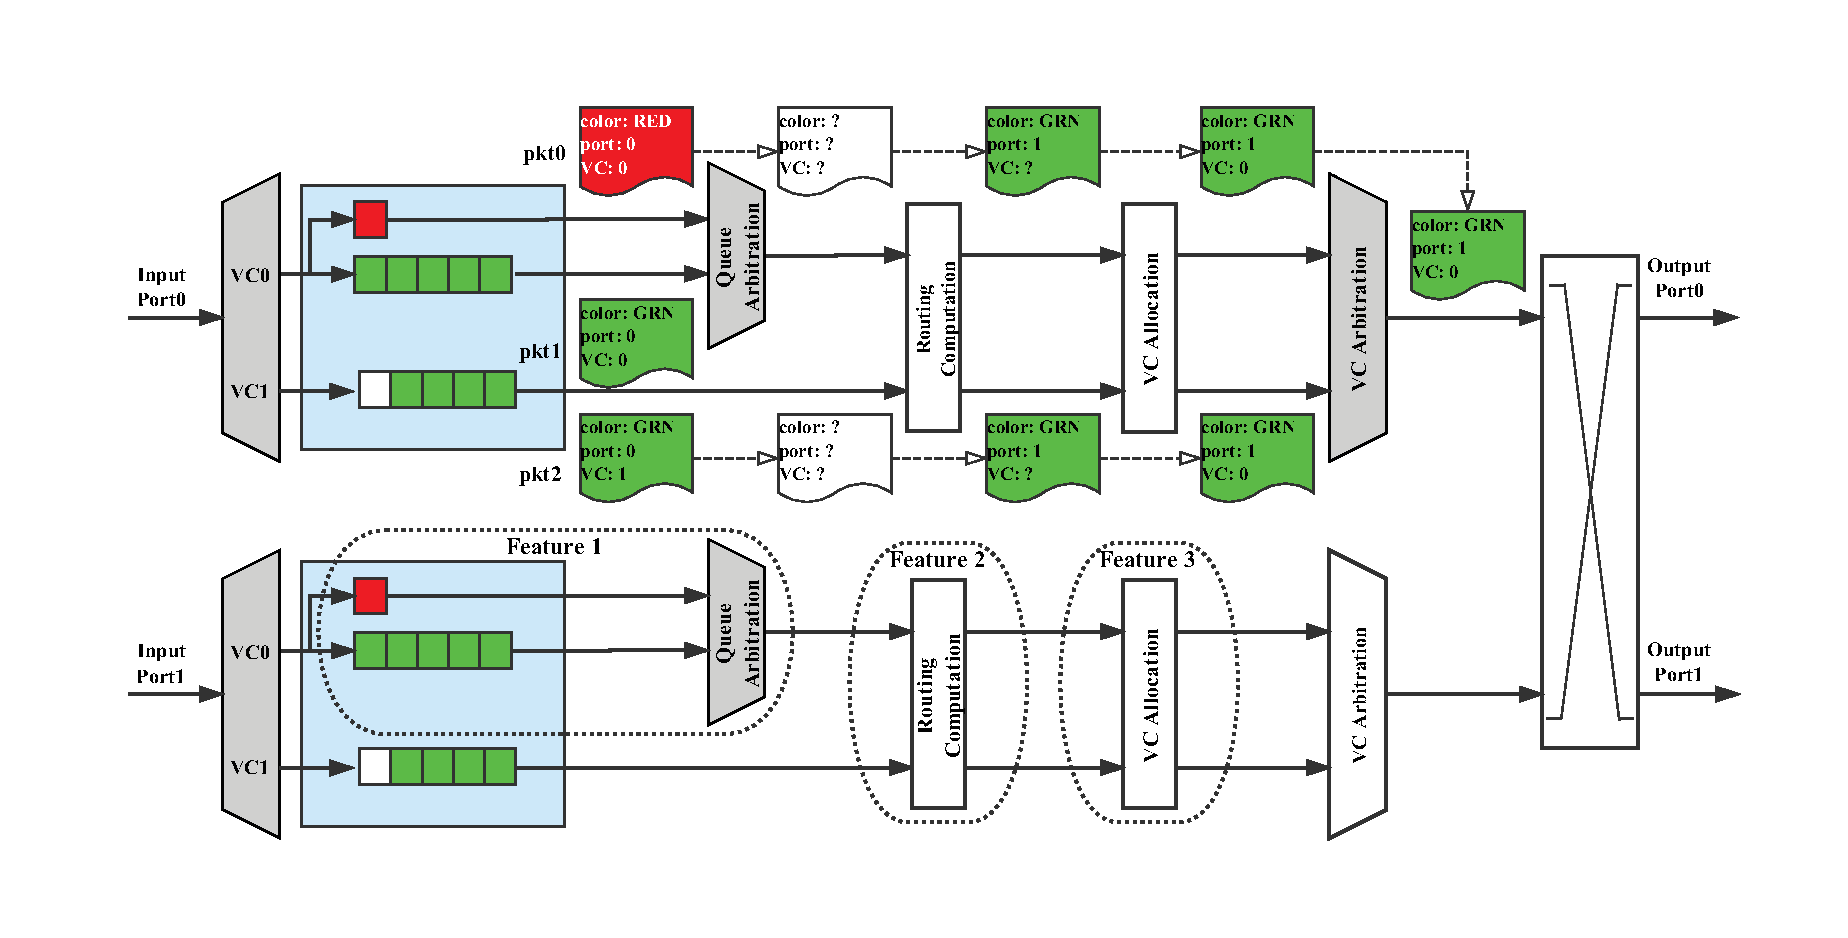
\includegraphics[width=.95\textwidth]{overview.eps}
  \caption{LBBO结构和LBR的工作流程}
  \label{fig:overview}
\end{figure*}

\section{LBR设计细节}

这一章节将要详细介绍Label-based Buffer Organization(LBBO)和它所支持的路由机
制LBR,其中包括路由计算模块和VC分配模块。

\subsection{Label-based Buffer Organization}

输入缓冲区是路由器微体系结构里最复杂的部分之一。特别是对于IQ路由器,
下游的输入缓冲区能够替代上游的输出缓冲区\upcite{PPIN}。当一个报文切片到达的
时候,它先进入输入缓冲区并滞留在那直到传输到下一跳路由器。

一般来说,输入缓冲区贯穿整个路由器,被静态划分或者使用链表动态划分为物理输入队列或者划分为多个VC\upcite{PPIN}。
Label-based Buffer Organization(LBBO
)是一种新的高阶路由器输入缓冲区设计。图\ref{fig:overview}展示了LBBO的框
架。LBBO的特点在于一个特别的缓冲区结构$VC_0$,Label-based FIFO。 Label-based
FIFO 由两个FIFO队列组成,一个小容量的负责存储上游路由器的红色报文队列和一个大容量的负责存储上游路由器的绿色报文的队列。
图\ref{fig:grbofifos}展示了两种Label-based FIFO的实现方法。图\ref{subfig:grbofifos-0}中两个FIFO 队列和
它们的控制器都是标准化的。唯一跟传统不一样的部件就是VC的控制器,其要连接
两个FIFO控制器。如果存放红色报文的队列足够小到职能容纳一个报文,那么,存
放红色报文的队列可以直接用寄存器代替,而相应的FIFO控制器可以省略,正如图
\ref{subfig:grbofifos-1}所示如果路由器提供多条VC,那么除了$VC_0$,其他VC
都被用来存放绿色报文就跟传统路由器结构的VC存放报文一样。如图\ref{fig:overview} 所示,
每个端口有两条VC。

在LBR机制中,红色报文使用的是无死锁路由算法而绿色报文则使用的是自适应
路由算法。因此,我们设计Dragonfly路由算法只需要使用一条VC,既不需要牺牲
路径的多样性,也最小化死锁避免的开销。$VC_0$的队列仲裁取决于红色队列是否
为空,如果红色队列有报文则赢得仲裁机会。

LBBO的设计特点有两个好处:(1)最小化死锁开销。因为在LBBO中,死锁避免不需要其他VC,$VC_0$同时被无死锁路由算法和自适应路由算法共享。整个设计只需要1 条
VC就可以实现无死锁的自适应路由,物理链路不需要复用。死锁避免的唯一开销就
是$VC_0$的红色队列,红色队列长度可以小到只需容纳一个报文的寄存器。相比
传统的经典路由器结构,尽管LBBO的$VC_0$的VC控制器要相对复杂一些和添加了color类型的标记位,但是相比减少额外的VC和相关控制信息,LBBO高效了利用
有限资源。同时,相比动态分配的多队列缓冲区管理,LBBO并没有消耗更多的资源。(2)最大化自适应性。LBR路由算法在下游路由器的缓冲区还有资源时,LBR
会优先选择自适应路由算法。在LBBO中,大部分输入缓冲区资源都是分配给存放
绿色报文的队列,使得更多的报文可以走自适应路由。而且,在Dragonfly这类大规
模低直径的网络中,死锁发生的概率很小\upcite{Warnakulasuriya2000A}。因此,
$VC_0$被自适应路由算法和无死锁路由算法共享,$VC_0$几乎不会成为系统的瓶颈。

\begin{figure}[t]
  \centering
  \subfloat[]{
    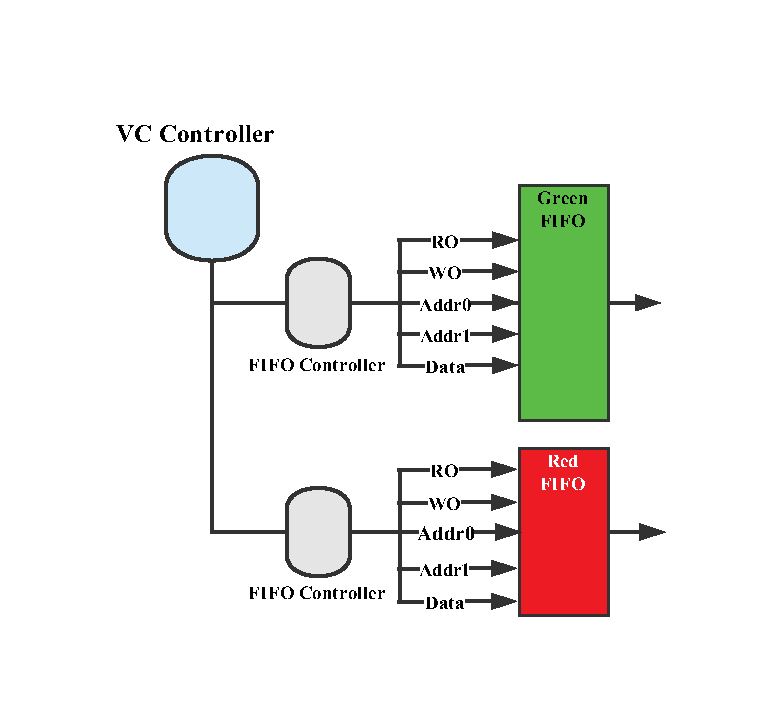
\includegraphics[width=.42\textwidth]{fifos-0.eps}
    \label{subfig:grbofifos-0}
  }
  \subfloat[]{
    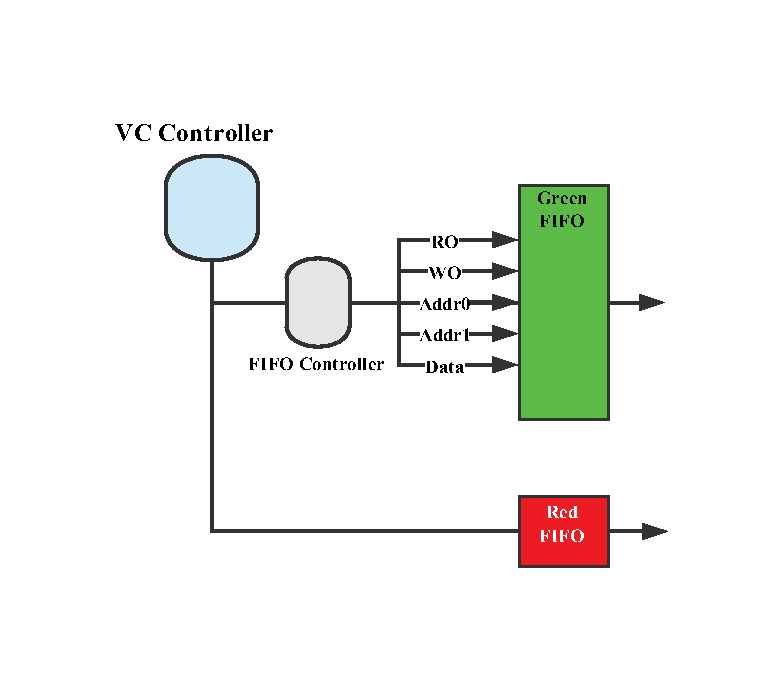
\includegraphics[width=.42\textwidth]{fifos-1.eps}
    \label{subfig:grbofifos-1}
  }
  \caption{Label-based FIFOs的实现}
  \label{fig:grbofifos}
\end{figure}

\subsection{Label-based路由算法}


路由算法为每一个报文计算输出端口和颜色类型。在这一小节中,我们详细介绍
Label-based路由算法(LBR)。LBR是一个混合路由算法,既可以执行完全自适应路由算法$LBR_A$也可以执行无死锁路由$LBR_D$。

路由计算模块由两个阶段组成。在第一阶段中,两个输出端口,$port\textrm{-}a$ 和$port\textrm{-}d$,分别由$LBR_A$ 和$LBR_D$计算所得。在第二阶段中,路由端口的最
终决策根据$port\textrm{-}a$和$port\textrm{-}d$所连接的下游路由器缓冲区状态决定。

自适应路由算法$LBR_A$如算法\ref{algo:ada}所示。每一个报文$pkt$到达
当前路由器,$LBR_A$计算输出端口$port-a$给报文。$LBR_A$先检查当前路由器
是不是目的节点的路由器,如果是则立即返回相应的输出端口(行1-行5)。如果
$pkt$需要被转发,$LBR_A$先计算最短路径的出口$port_{min}$(行6)。对于每一个输出端口$port_i$,路由器有两个计数器,$green_i$和$red_i$,负责统计$port_i$所连接的下一级路由器的输入端口红色报文和绿色报文的数量情况。如果
最短路径的绿色报文$green_{min}$小于设定的阈值$T_{min}$,那么$port_{min}$
作为输出端口,而$pkt$则路由走最短路径路由(行7-行8)。否则,$LBR_A$检测
所有绿色报文计数器小于$T_{non-min}$的非最短路径而且收集他们相对应的输出端
口到集合$P$(行10)。如果$P$不是空集,$LBR_A$则随机选择一条非最短路径(行11-行12),否则最短路径的端口$port_{min}$被选择并返回(行13-行14)。最后,路由结构被返回(行17)。在算法\ref{algo:ada} 中,阈值$T_{min}$ 和$T_{nonmin}$都是基于反复实验调整所得的经验值。在$LBR_A$中,最短路径路由优
先,因为最短路径可以降低网络延迟。在策略中,可能有比随机选择非最短路径路由有更好的办法,但是随机的方法简单且可以获得较好的性能。


\begin{algorithm}[t]
  \centering
  \caption{自适应路由算法}
  \label{algo:ada}
  \begin{algorithmic}[1]
    \REQUIRE 报文 $pkt$
    \ENSURE 自适应路由的输出端口 $port\textrm{-}a$
    \STATE $R_{dest} \leftarrow 目的路由器编号(pkt)$
    \IF {$R_{dest} = 当前路由器编号$}
    \STATE $port\textrm{-}a \leftarrow 终端端口$
    \RETURN $port\textrm{-}a$
    \ENDIF
    \STATE $port_{min} \leftarrow 最短路径(R_{dest})$
    \IF {$绿色报文计数器{port_{min}} < T_{min}$}
    \STATE $port\textrm{-}a \leftarrow port_{min}$
    \ELSE
    \STATE $P \leftarrow \{port_i\ |绿色报文计数器{port_i} < T_{non\textrm{-}min}, i \in [0,4h-2], i \neq min\}$\hspace{-1em}
    \IF{$P \neq \emptyset$}
    \STATE $port\textrm{-}a \leftarrow 随机选择(P)$;
    \ELSE
    \STATE $port\textrm{-}a \leftarrow port_{min}$;
    \ENDIF
    \ENDIF
    \RETURN $port\textrm{-}a$
  \end{algorithmic}
\end{algorithm}

对于$LBR_D$,我们采用基于树型的无死锁路由算法\upcite{Survey}\upcite{OFAR-CM},每一个报文都是经过自上而下的已有的路径到达所有路由器节点。在Dragonfly结构中,随机选取一个路由器节点作为根节点$R_{root}$而$R_{root}$所在的超级节点作为根超级节点$G_{root}$。在$G_{root}$中的每一个路由器节点都连接一个或几个其他超级节点内的路由器节点。这些被根超级节点相连在其他超级节点的路由器节点再通过
本地链路连接同一个超级节点内的其他节点。

第一阶段计算出$port\textrm{-}a$ 和$port\textrm{-}d$之后,LBR必须选择其中一个作为最后的输出端口。算法\ref{algo:greenred}展示了LBR是如何选择最终的
路由决策。首先,$port\textrm{-}a$ 和$port\textrm{-}d$在第一阶段计算后被获
取到(行1-行2)。如果$port\textrm{-}a$所对应的下游路由器端口的输入缓冲区
绿色队列还没有满,那么最终端口选择$port\textrm{-}a$而且$pkt$被标记为绿色(行3-行4)。否则,如果$port\textrm{-}d$所对应的下游路由器端口的输入缓冲区绿色队列还没有满,那么最终端口选择$port\textrm{-}d$而且$pkt$被标记为绿色(行5-行6)。否则,最终输出端口选择$port\textrm{-}d$而且$pkt$被标记为红色(行7-行8)。我们阻止一个红色报文在同一个超级节点内变为绿色报文(行10- 行12),因为一个报文在同一个超级节点内频繁改变颜色类型容易造成活锁。那
么,根据报文的颜色类型更新相应的报文计数器(行13-行17)并返回端口和颜色类
型的结果(行18)。算法\ref{algo:greenred}在执行的时候优先使用自适应路由算
法。当网络非常拥塞的时候即$port\textrm{-}a$ 和$port\textrm{-}d$都不能提供
绿色报文队列的缓冲区时,报文才会被标记为红色。

\begin{algorithm}[t]
  \centering
  \caption{LBR路由算法}
  \label{algo:greenred}
  \begin{algorithmic}[1]
    \REQUIRE 报文 $pkt$
    \ENSURE 输出端口和颜色类型 $(port, color)$
    \STATE $port\textrm{-}a \leftarrow adaptive\_port(pkt)$
    \STATE $port\textrm{-}d \leftarrow deadlockfree\_port(pkt)$
    \IF {$green{port\textrm{-}a} < T_{green}$}
    \STATE $(port, color) \leftarrow (port\textrm{-}a, GREEN)$
    \ELSIF {$green_{port\textrm{-}d} < T_{green}$}
    \STATE $(port, color) \leftarrow (port\textrm{-}d, GREEN)$
    \ELSE
    \STATE $(port, color) \leftarrow (port\textrm{-}d, RED)$
    \ENDIF
    \IF {$color = GREEN$ \textbf{and} $get\_color(pkt) = RED$ \textbf{and}
      $supernode(port) = my\_supernode\_id$}
    \STATE $(port, color) \leftarrow (port\textrm{-}d, RED)$
    \ENDIF
    \IF {$color = GREEN$}
    \STATE $green_{port} \leftarrow green_{port} + 1$
    \ELSE
    \STATE $red_{port} \leftarrow red_{port} + 1$
    \ENDIF
    \RETURN $(port, color)$
  \end{algorithmic}
\end{algorithm}

为Dragonfly结构设计的Label-based路由算法能够避免死锁。假设Dragonfly结构中
有一个环,这样的环依赖于链路$a->b$和$b->a$。在Dragonfly结构中$a->b$的依赖
被无死锁路由允许但是$b->a$则不被允许。当报文存储在端口B的输入缓冲区并被标记为绿色,申请去输出端口A。当网络发生死锁,报文在一个环中不能转发到下游路由器。这意味着环上的缓冲区已满。这种情况,意味着环路上的缓冲区全部存放着绿色报文,当下游路由器存放绿色报文的队列还有空
余位置,报文的颜色类型才会标记为绿色。否则,报文标记为红色的话,报文则不会走带环的路径。因此,这种情况不可能存在。网络中不会出现报文堵塞在依赖环
中。尽管绿色报文可以走任意路径,但是红色报文走的是无死锁路由。

例如,在图\ref{fig:deadlockfree}中,Dragonfly结构有三个超级节点,每个超级
节点内有两个路由器节点。每个路由器都跟相邻的超级节点的路由器节点发信息,
即每个路由器都跟右边隔两个编号的路由器节点通信。路由节点$R_0$的输入缓冲区
里绿色队列里有两个$R_5$到$R_1$的报文,红色队列里有一个报文是从无死锁路径
上与$R_0$相邻的路由器转发的。$R_5$到$R_0$没有直接的无死锁路径,所以从$R_5$去$R_1$的报文进入绿色队列。 $R_1$ 的3个
报文都是从$R_0$到$R_2$。一个报文在红色队列中是按无死锁路由从
从$R_0$到$R_1$。$R_2$、$R_3$和$R_4$的情况跟$R_1$一样。$R_5$
有两个从$R_4$到$R_0$的报文在绿色报文队列中。因为$R_4$到$R_0$
经过$R_5$,所以这条路径不是无死锁路径。因为绿色队列没有空余的
缓冲区资源,所以$R_4$ 不能再发送其他
报文给$R_0$经过$R_5$。那么,所有报文都可以继续传输,因为$R_5$
缓冲区的红色队列是空余的,不受限于绿色队列形成的环路。

\begin{figure*}[t]
  \centering
  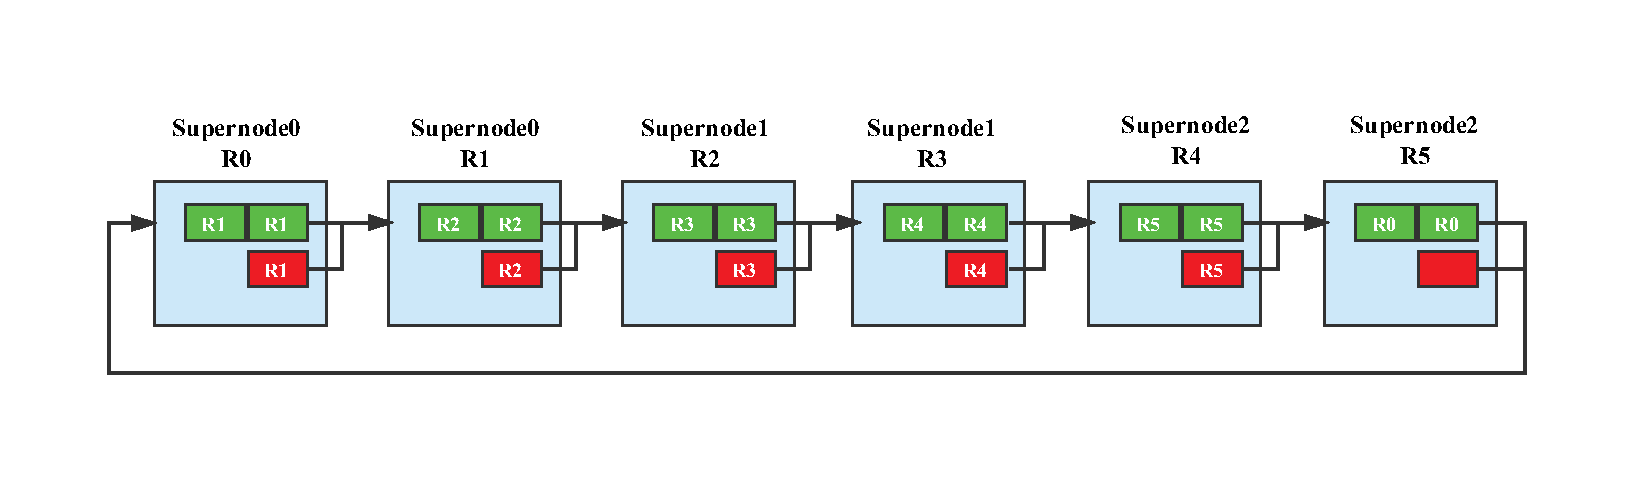
\includegraphics[width=.95\textwidth]{deadlockfree_prove.eps}
  \caption{Dragonfly的死锁避免机制范例}
  \label{fig:deadlockfree}
\end{figure*}

LBR的优势:(1)在有限的缓冲区资源条件下,尽可能的最大化路由的自适应性。
(2)在$LBR_A$中,在性能不受影响下,有效的优先选择最短路径路由。

\subsection{VC分配模块}


VC分配模块的任务是给每一个报文安排一个VC。然而,在Dragonfly结构中,路由算法使用VC隔离固定使用VC 的顺序来避免死锁发生。
这样,VC分配就会在路由计算模块就已经确定了
VC的分配。在LBR中,死锁避免对VC没有额外的限制,因此,绿色报文可以选择不同的VC。

为了均衡存放绿色报文队列的利用率,我们提出三种分配VC的方案:
随机选取(Random),最短长度选取(Minimal)以及模运算最短长度选取(Mod-Minimal)。

随机选取策略是最简单的策略,即随机的给报文选取一条VC。
最短长度选取则是在存放绿色报文队列中的VC里选取剩余最多空余位置的VC。
模运算最短长度选取作为默认的策略如算法\ref{algo:va}所示。在选择最短长度
的VC前,VC的分配器根据报文已经经过几个超级节点做一个模运算。

算法\ref{algo:va}展示了模运算最短长度选取策略。红色报文直接分配$VC_0$(行1-行3)。
一个VC被分配给绿色报文,首先,获得报文的路由端口(行4)。报文有一个$hop$ 域用来记录
报文已经路由经过几个超级节点(行5)。$hop$值的更新取决于报文的位置。路由器为每一个输出端口都维护了一个常数值$nqueues_{port}$,即存放绿色报文队列划分成VC的数量。这个设计不需要额外的硬件开销。其中一条VC被分配给报文。变量$modq$记录了
$hop$模$nqueues_{port}$的运算结果(行6)。第$modq$条VC如果还有剩余的空位(通过$credit_{port}^{modq}$统计返回相关值),则该条VC被分配给报文(行7- 行8)。否则,最短长度的队列
即空余位置最多的VC被分配给报文(行9-行10),同时更新$credit_{port}^{modq}$的值(行12)。最后将分配的VC编号返回给报文(行13-行14)。

VC分配模块实际上就是给绿色报文分配一个合适的队列。通过模运算选取VC相比直接选取
最短长度的VC效果更好主要原因是因为考虑了报文的状态,对报文做了划分,不仅
降低了头阻塞的概率并一定程度上缓解了对最短长度
VC的竞争。模运算最短长度选取只需要一些报文信息和每条VC的信用值,相比
最短长度选取VC的策略不需要额外的硬件开销。

\begin{algorithm}[t]
  \centering
  \caption{VC分配机制}
  \label{algo:va}
  \begin{algorithmic}[1]
    \REQUIRE 报文 $pkt$
    \ENSURE 虚拟通道  $VC$
    \IF {$颜色类型(pkt) = RED$}
    \RETURN $0$
    \ENDIF
    \STATE $port \leftarrow 路由端口(pkt)$
    \STATE $hop \leftarrow 经过超级节点的跳步数(pkt)$
    \STATE $modq \leftarrow hop\ \textbf{mod}\ nqueues_{port}$
    \IF {$credit_{port}^{modq} > 0$}
    \STATE $queue \leftarrow modq$
    \ELSE
    \STATE $queue \leftarrow max\_credit\_queue(port)$
    \ENDIF
    \STATE $credit_{port}^{modq} \leftarrow credit_{port}^{modq} + 1$
    \STATE $VC \leftarrow associated\_vc(queue)$
    \RETURN $VC$
  \end{algorithmic}
\end{algorithm}

\section{评估分析}

在这一节中,我们使用基于时钟精确的模拟器Booksim评测了不同的路由算法。
模拟配置总结如下。

\textbf{路由器:}我们采用基于LBBO缓冲区管理和支持LBR新的路由器微体系结构。
其他路由算法采用的则是经典的输入队列(IQ)路由器结构并执行完整的路由器流水线步骤。
我们假设在两个路由器结构中信用处理均需要2个时钟周期,路由计算模块2个时钟周期,
交换分配以及VC 分配以及crossbar处理分别需要1个时钟周期。输入和输出的crossbar加速比
均为1,但是 路由器内部链路的速率则是片间链路传输延迟的2倍。

\textbf{网络:}负载均衡的Dragonfly结构可以用参数$h$定义\upcite{dragonfly}。
整个网络是由$2h^2+1$个超级节点组成的全互连网络,而每一个超级节点则是由$2h$
个路由器节点组成的全互连网络。每个路由器的端口数为$4h-1$,其中$h$个端口连接终端,
$h$个端口连接其他超级节点,$2h-1$条链路连接超级节点内部的路由器。
我们模拟评测的是$h=4$的Dragonfly结构,规模为1056个路由终端。为了区分本地链路和全局链路,
我们设置本地链路传输延迟为50个时钟周期,而全局链路则设置为100个时钟周期。
本地端口的缓冲区设为144个切片大小,而全局端口的缓冲区则设为256个切片大小。
缓存资源采用静态划分方式,每个VC的大小相同。针对$VC_0$,缓存资源由红色队列和绿色队列
共享,但是红色队列只占有1个报文大小。我们使用报文作为测量单位。其他报文长度(如:16个切片大小)和
其他全局端口的缓冲区大小(如:128个切片大小)都被分析了。所有统计的结果都是在预热阶段之后
网络进入稳定之后收集的。

\textbf{路由算法:}我们比较以下路由算法:最短路径路由(MIN),基于节点的非最短路径路由(VAL$_n$),
全局负载均衡自适应路由算法(UGAL),主动自适应路由算法(PAR),投机的本地绕路路由算法(OLM),
受限制的本地绕路路由算法(RLM)和Label-based路由算法(LBR)。对于LBR,路由路径被限制在8跳以内。
$T_{green}$ 和 $T_{red}$(在算法\ref{algo:greenred}中与绿色队列和红色队列中的切片数量比较)
的阈值分别设置为143(全局端口则为255)和1(全局端口则为1)。通过多次评测,$T_{min}$ 和 $T_{nonmin}$
(在算法\ref{algo:ada}中缓冲区占有率的百分比)设为0.8和0.5。在模拟评测时,为了与
其他路由算法公平比较,分别评测了LBR拥有1条VC(LBR-1)、2条VC(LBR-2)和3 条VC(LBR-3)的性能。
我们详细评测了不同的VC分配策略(Random、Mod-Minimal和Minimal)的性能。Mod-Minimal分配策略是
默认的分配策略。

\textbf{通信模式:}我们模拟了多个典型高性能计算工作负载。我们测试了图计算、稀疏线性代数求解以及
自适应mesh搜寻等应用里常出现的随机通信模式\upcite{Yuan}\upcite{slimfly}。我们也测试了stencil工作负载
的典型通信模式按位取反和位变换的通信模式\upcite{Yuan}。另外,还测试了具备Dragonfly结构
特点的最差通信模式以及全局通信模式\upcite{OFAR}。最后,我们针对Dragonfly结构设计了一种混合通信模式
来模拟测评Dragonfly在混合工作负载下的性能。


\subsection{随机通信模式}

在随机通信模式下,每个报文的源节点和目的节点都是随机选取。图\ref{latency1flit4pattern0}和图\ref{latency1flit4pattern1}
展现了随机通信模式下网络延迟和吞吐率。LBR-2的性能是最好的,延迟和吞吐率分别优于排在第二位的MIN路由算法$10\%$ 和
$20\%$。LBR-2跟MIN一样,选择最短路经路由,而且LBR-2可以均衡地分配2条VC的缓存资源。
而MIN,因为死锁避免策略,选择VC必须按照固定顺序,不能均衡VC利用率。
VAL$_n$在注入率为0.45的时候饱和,主要原因是最短路径几乎不使用而且绕路路径是
最短路径得两倍,因此饱和吞吐率受限制。PAR使用的VC数量是所有路由算法最多的,因为
缓存资源是有限的,那么分配给每条VC的资源有限,所以性能下降严重。
UGAL、RLM以及OLM三种路由算法都是使用3条VC来避免死锁,但是它们性能均不同,
主要因为他们的自适应的策略。


\begin{figure*}[htbp]
  \centering
  \begin{minipage}[t]{\textwidth}
  \centering
  \subfloat[Latency]{
    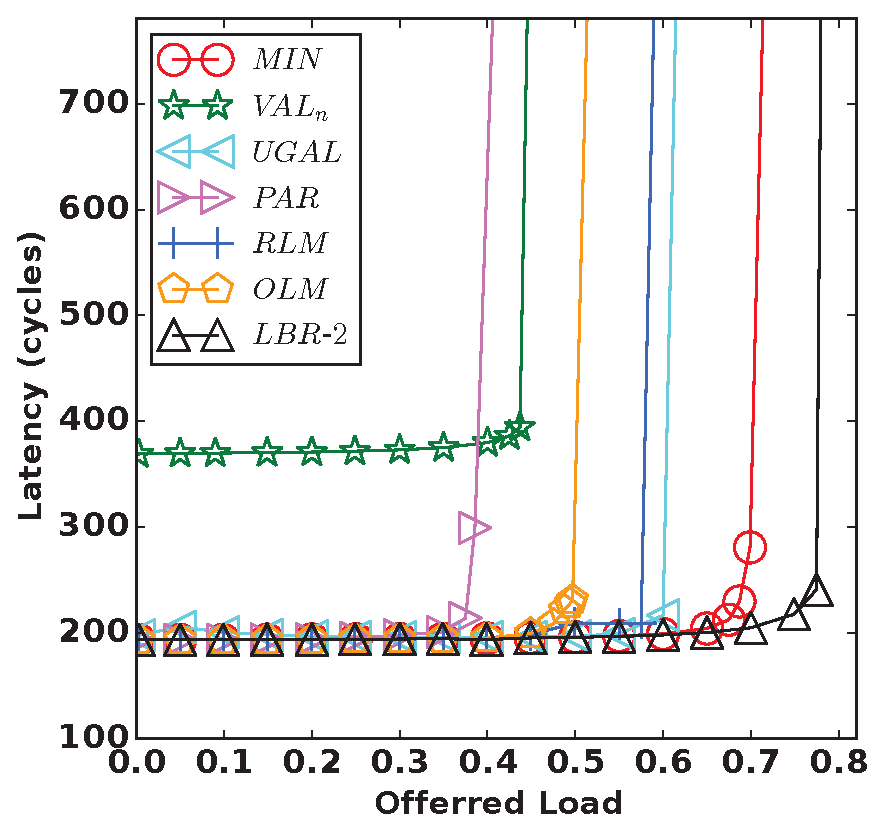
\includegraphics[width=.40\textwidth,height=.42\textwidth]{latency1flit4pattern0.eps}
    \label{latency1flit4pattern0}
  }
  \subfloat[Throughput]{
    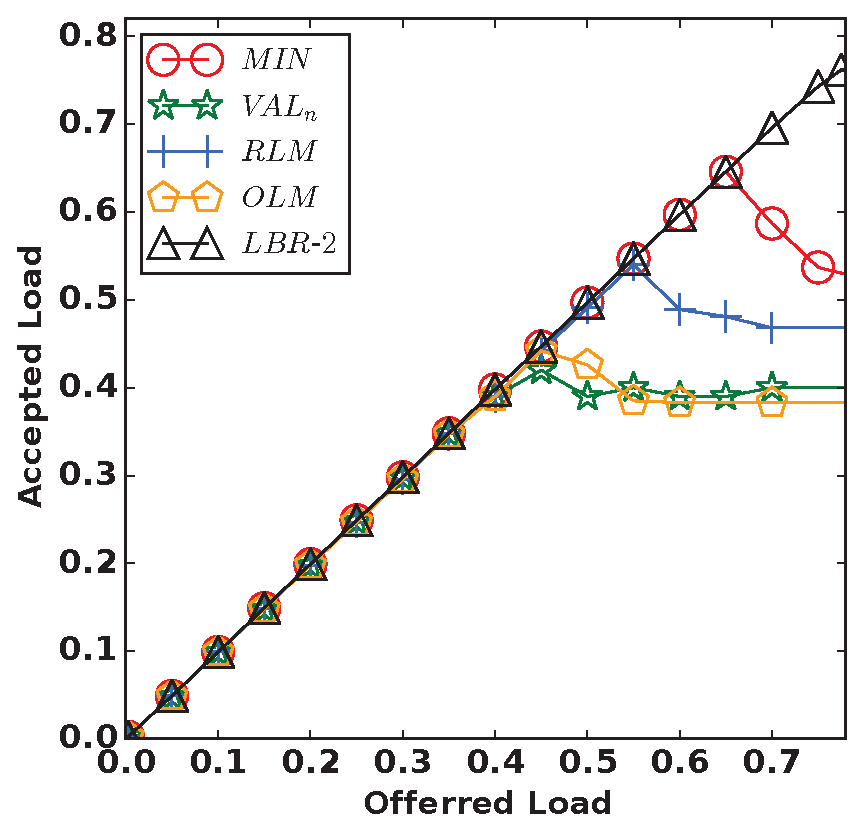
\includegraphics[width=.40\textwidth,height=.42\textwidth]{throughput1flit4pattern0.eps}
    \label{throughput1flit4pattern0}
  }
  \caption{均衡随机通信模式}
  \label{fig:random}
  \end{minipage}
  \end{figure*}

\subsection{位取反和位变换通信模式}

我们评测了LBR-2路由算法在位取反和位变换的通信模式下的网络延迟和吞吐率。$b$为每个终端地址的位数,
$s_i$是源节点的第$i$位地址而$d_j$则是目的节点的第$j$位地址。位取反和位变换通信模式要求网络规模
是2的幂次方大小。在Dragonfly结构中,因为规模不是标准的2的幂次方,则限制一些终端不能接收消息\upcite{slimfly}。 在$h=4$的Dragonfly结构里,1056个
终端中有32个终端只能发送消息不能接收消息。我们评测这两种通信模式的主要目
的是模拟集群通信的场景,位取反中目的节点和源节点的关系为$d_i=s_{b-i-1}$以及位变换中目的节点和源节点的
关系为$d_i=s_{(i+b/2) mod b}$。图\ref{fig:bitrev}和图\ref{fig:transpose} 分别展示了
位取反和位变换的性能。在两种通信模式下,MIN是最好的路由算法,获得最低的延迟和最高的吞吐率。
在位取反的通信模式下,LBR-2跟MIN的性能基本上是一致。在位变换的通信模式下,LBR-2在高负载的性能略低于
MIN的性能。RLM和OLM展现了相似的性能,在位取反通信模式下略低于$10\%$LBR-2 和MIN的性能。因为两倍的路径
长度,VAL$_n$在两个通信模式下都是最差的性能。



  \begin{figure*}[htbp]
  \centering
  \begin{minipage}[t]{\textwidth}
  \centering
  \subfloat[Latency]{
    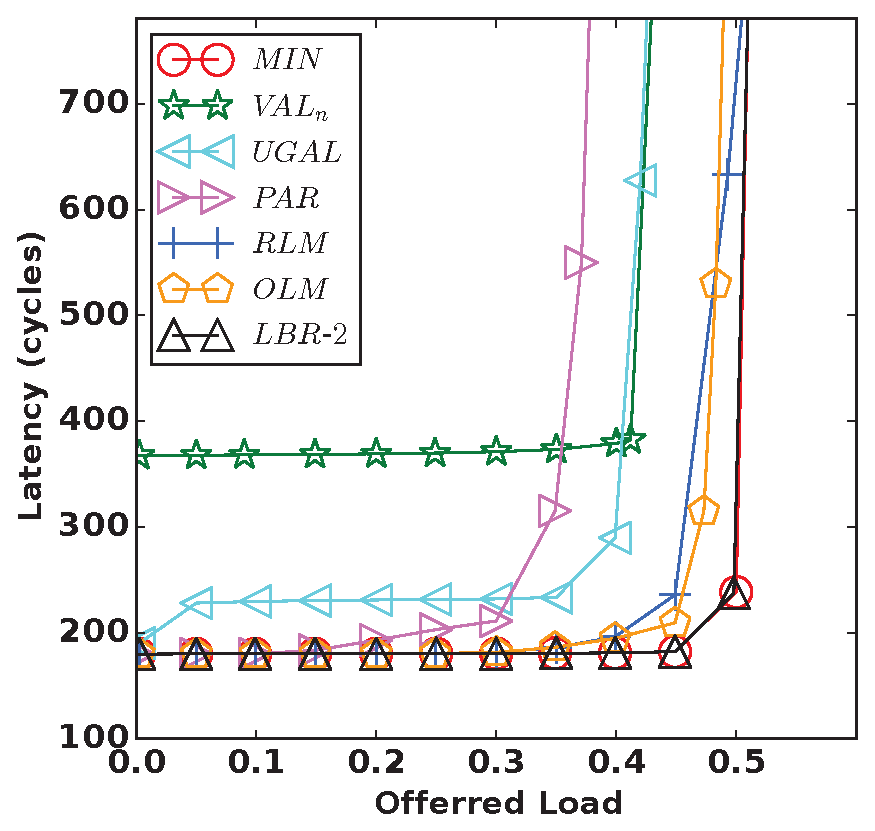
\includegraphics[width=.40\textwidth,height=.42\textwidth]{latency1flit4pattern1.eps}
    \label{latency1flit4pattern1}
  }
  \subfloat[Throughput]{
    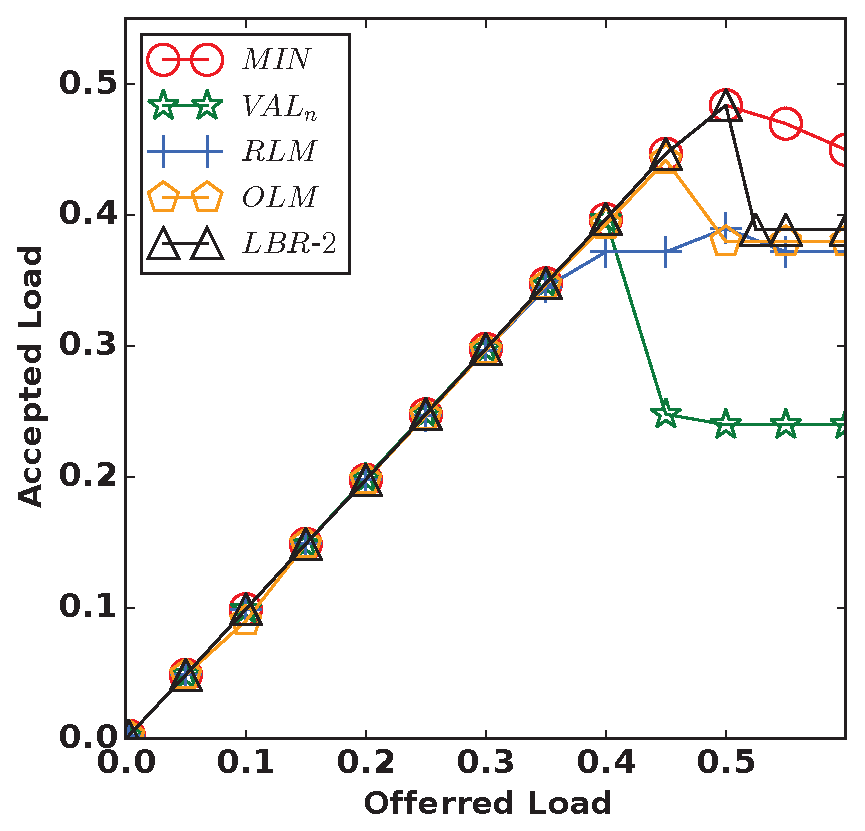
\includegraphics[width=.40\textwidth,height=.42\textwidth]{throughput1flit4pattern1.eps}
    \label{throughput1flit4pattern1}
  }
  \caption{位取反通信模式}
  \label{fig:bitrev}
   \end{minipage}
\end{figure*}


\begin{figure*}[htbp]
  \centering
  \begin{minipage}[t]{\textwidth}
  \centering
  \subfloat[Latency]{
    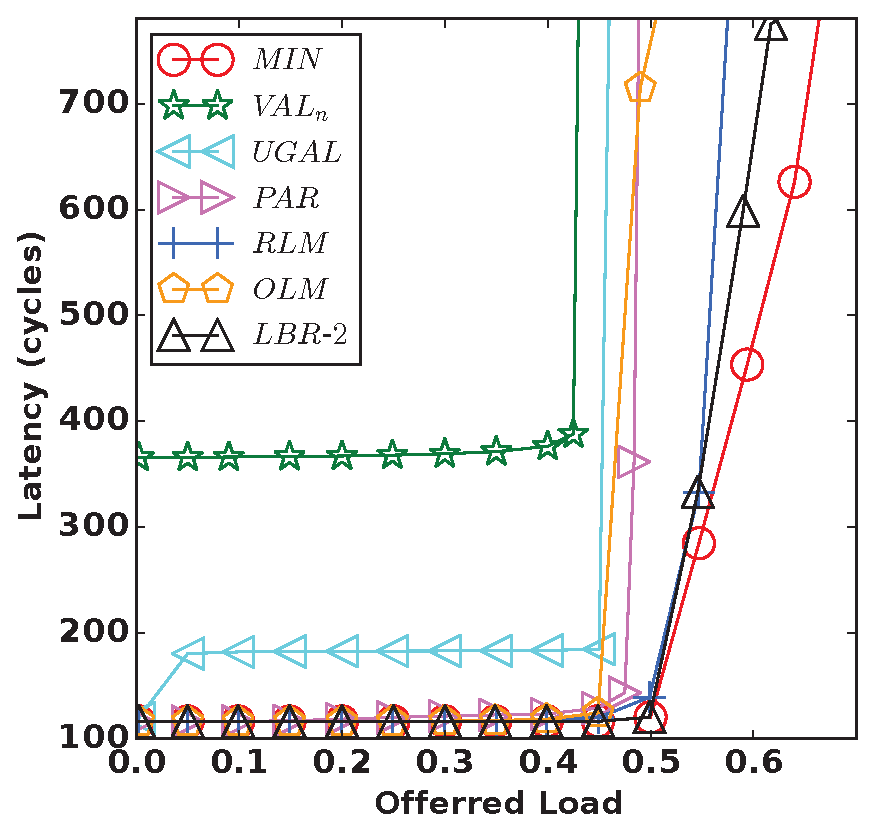
\includegraphics[width=.40\textwidth,height=.42\textwidth]{latency1flit4pattern2.eps}
    \label{latency1flit4pattern2}
  }
  \subfloat[Throughput]{
    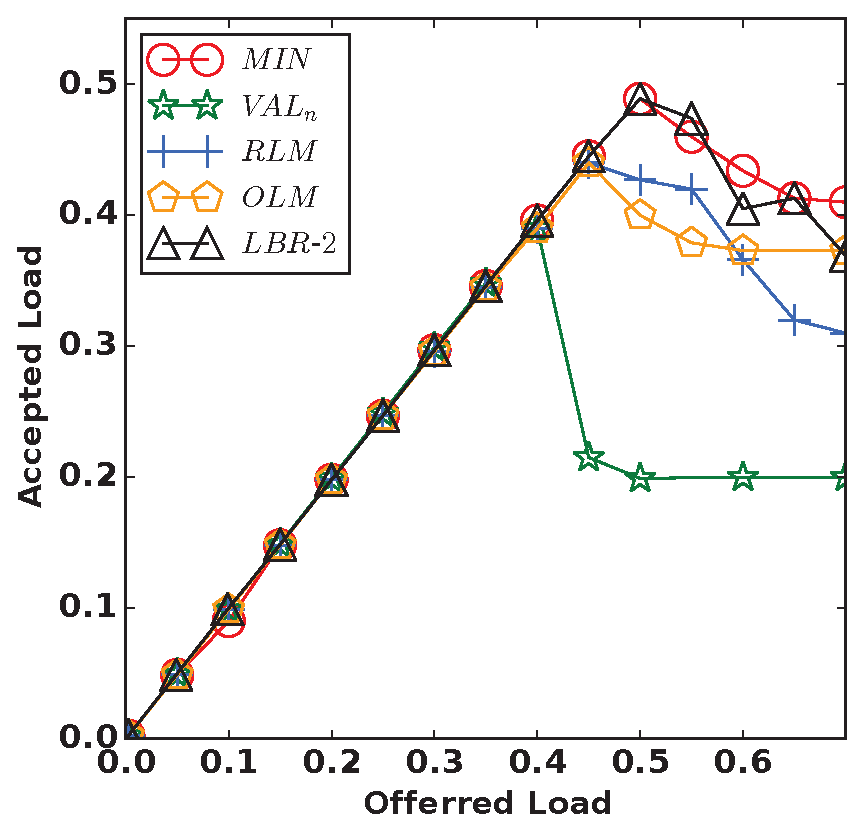
\includegraphics[width=.40\textwidth,height=.42\textwidth]{throughput1flit4pattern2.eps}
    \label{throughput1flit4pattern2}
  }
  \caption{位变换通信模式}
  \label{fig:transpose}
  \end{minipage}
  \end{figure*}



\subsection{全局和最差通信模式}


分析Dragonfly结构中超级节点之间的通信是非常重要的工作。因为,相比本地链路,全局链路数量上受限制,容易造成瓶颈。
另外,超级节点之间通信在实际系统部署上也是一类典型应用。因此,我们设计了全局通信模式和最差通信模式来
模拟分析不同路由算法是如何解决Dragonfly结构中超级节点之间的通信问题。
在全局通信模式下,终端只与其它超级节点的路由节点通信,不同路由算法的性能如图\ref{fig:global}所示。
LBR-2展现了最高的饱和吞吐率点而且获得了最低的网络延迟。当注入率大于0.5之后,延迟略微增加了$10\%$。因为
一些报文在高负载下开始执行绕路路由。因为RLM在超级节点内禁止一些路径的路由,
RLM的饱和吞吐率比OLM的饱和吞吐率低将近$12.5\%$。VAL$_n$的延迟是路由算法中最高的,主要原因还是
确定的绕路路由增加了路径长度(长度可达6跳)。


\begin{figure*}[htbp]
  \centering
  \begin{minipage}[t]{\textwidth}
  \centering
  \subfloat[Latency]{
    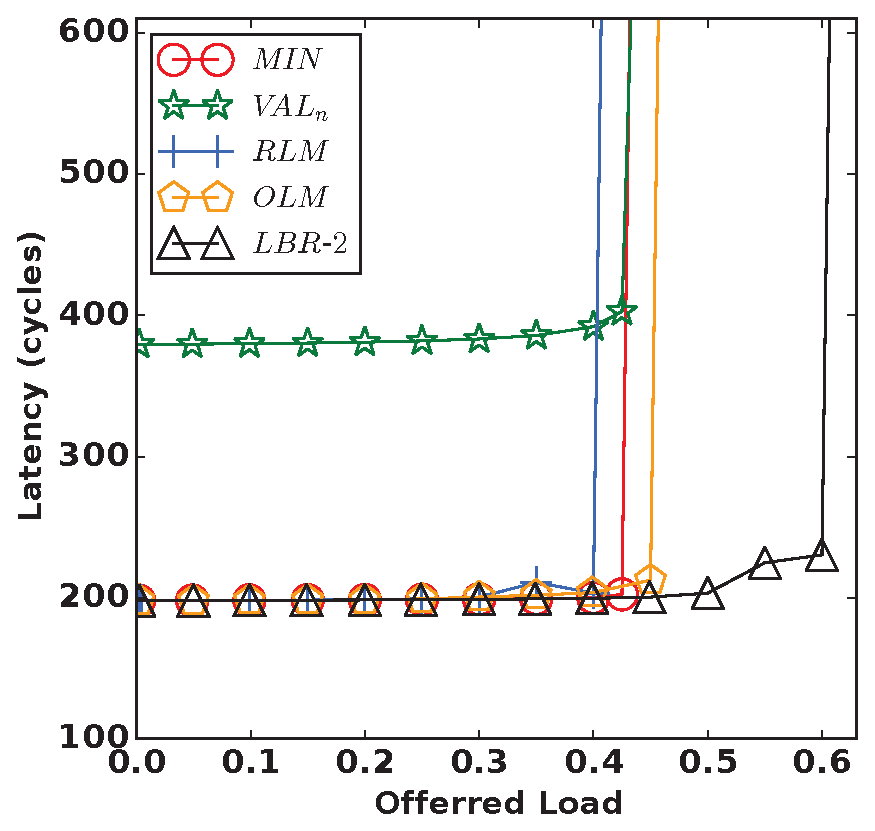
\includegraphics[width=.40\textwidth,height=.42\textwidth]{latency1flitinternal.eps}
    \label{latency1flitinternal}
  }
  \subfloat[Throughput]{
    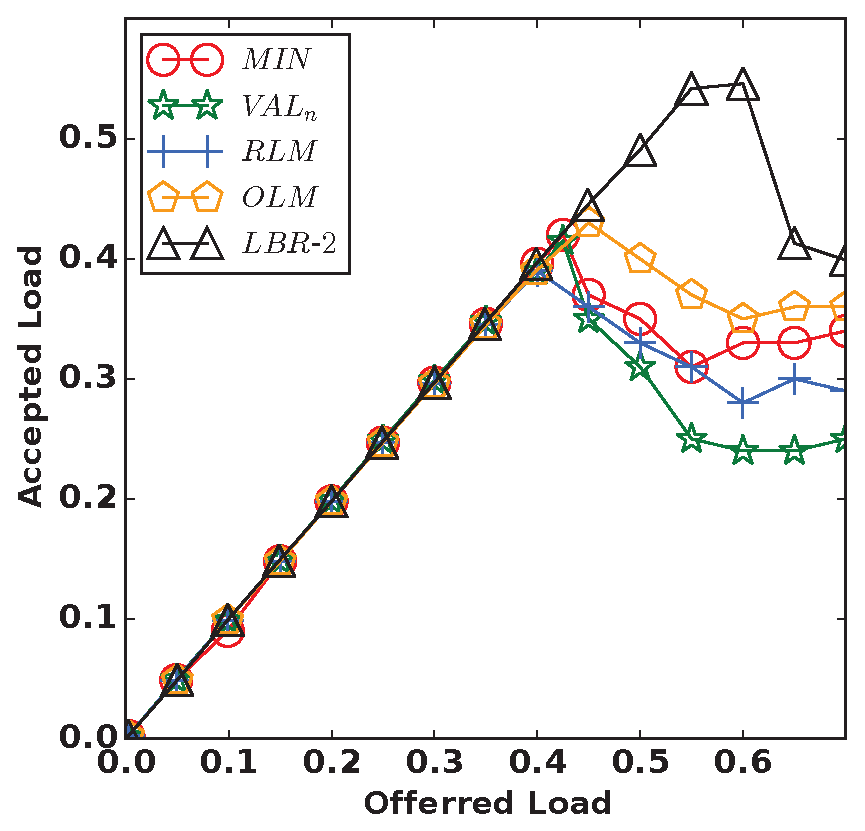
\includegraphics[width=.40\textwidth,height=.42\textwidth]{throughput1flitinternal.eps}
    \label{throughput1flitinternal}
  }
  \caption{全局通信模式}
  \label{fig:global}
  \end{minipage}
\end{figure*}

在最差通信模式下,每个超级节点内的路由节点都跟固定的超级节点的路由节点进行通信。
图\ref{fig:adversarial}展示了最差模式下的性能。在最差通信模式下使用MIN,网络
在低负载时就迅速饱和并拥塞。VAL$_n$则获得最高的性能,注入率能达0.3。VAL$_n$
不同于传统的VAL路由算法,每个报文都先路由到中介超级节点的中介路由节点,然后再
由中介路由节点走最短路径到达目的路由节点。这样可以较好的完成负载均衡以及避免
超级节点内部本地链路的瓶颈\upcite{overcomefarend}。但是,VAL$_n$相比传统的VAL
路由算法还需要多一条VC来避免死锁。RLM相比LBR-2,不仅有较高的饱和吞吐率而且获得较低的延迟。
但是,LBR-2的性能比OLM、PAR以及UGAL的都要更优。


\begin{figure*}[htbp]
  \centering
   \begin{minipage}[t]{\textwidth}
  \centering
  \subfloat[Latency]{
    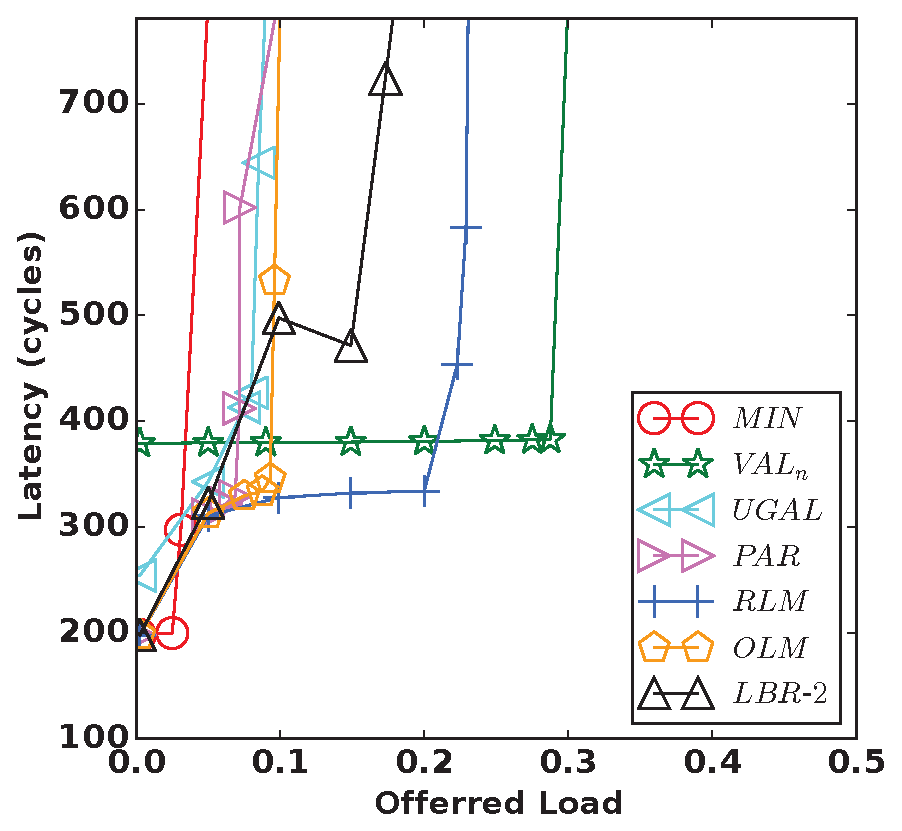
\includegraphics[width=.40\textwidth,height=.42\textwidth]{latency1flit4pattern3.eps}
    \label{latency1flit4pattern3}
  }
  \subfloat[Throughput]{
    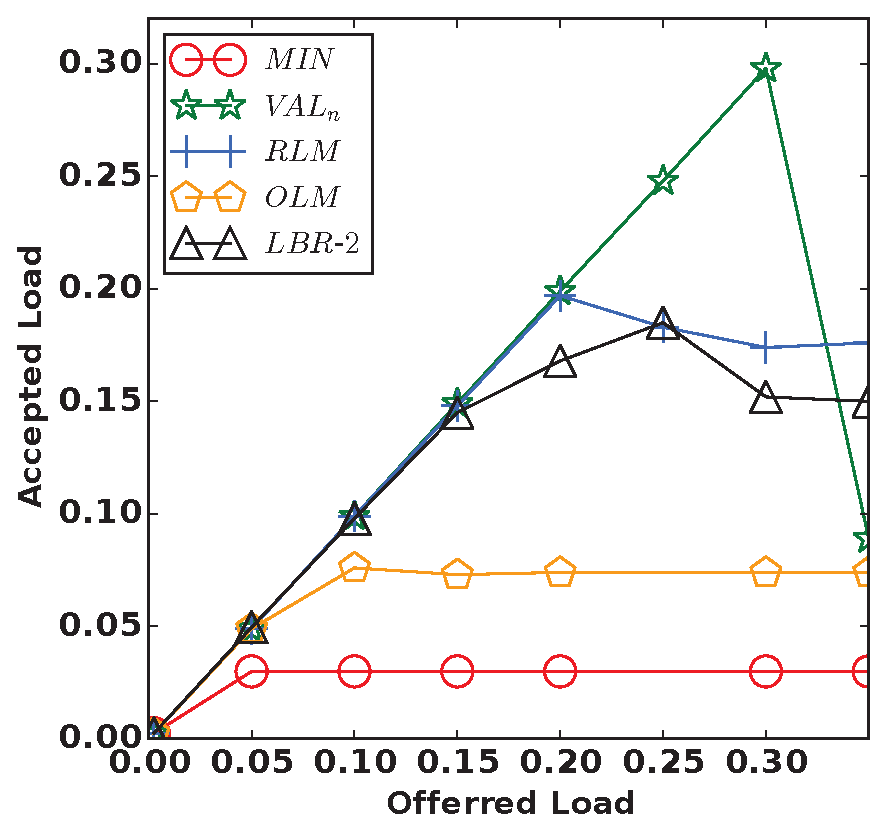
\includegraphics[width=.40\textwidth,height=.42\textwidth]{throughput1flit4pattern3.eps}
    \label{throughput1flit4pattern3}
  }
  \caption{最差通信模式}
  \label{fig:adversarial}
  \end{minipage}
  \end{figure*}


\subsection{混合通信模式}

在实际高性能计算系统中,大规模通信模式不是单一一种的,而是多种混合的。
因此,我们设计了一种混合的通信模式来模拟这些应用。Dragonfly
的混合通信模式采用90\%的随机通信模式和10\%的最差通信模式组成。
模拟结果如图\ref{fig:blended}所示。LBR-2获得了最高的性能。相比
其它路由算法,MIN的性能最差。主要原因是因为全局链路的拥塞导致
性能急剧下降。OLM的性能优于RLM,因为RLM的路径多样性低于OLM。
虽然VAL$_n$的路径长度是别的路由算法的两倍,但是,VAL$_n$因为
绕路避免了部分网络拥塞提高了饱和吞吐率。


  \begin{figure*}[htbp]
  \centering
  \begin{minipage}[t]{\textwidth}
  \centering
  \subfloat[Latency]{
    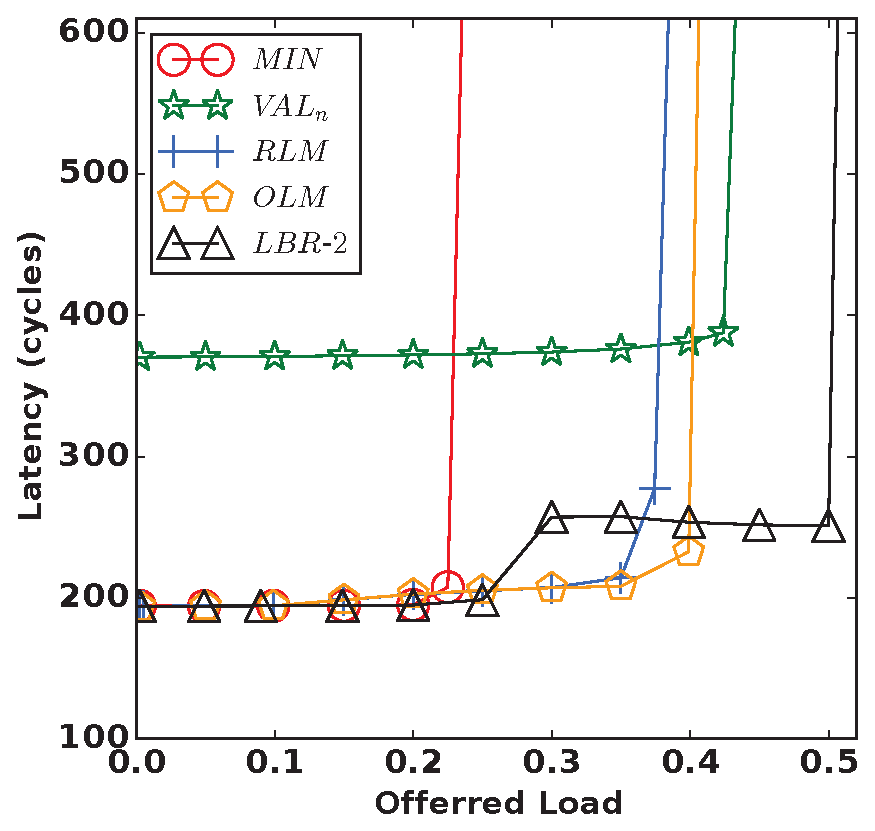
\includegraphics[width=.40\textwidth,height=.42\textwidth]{latency1flitblend.eps}
    \label{latency1flitblend}
  }
  \subfloat[Throughput]{
    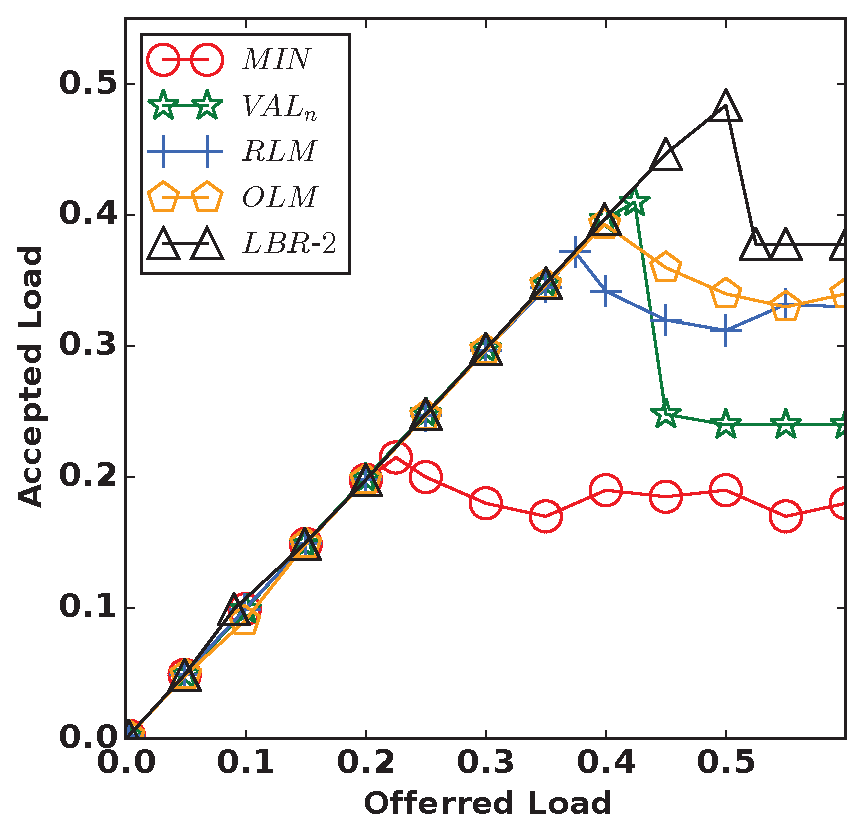
\includegraphics[width=.40\textwidth,height=.42\textwidth]{throughput1flitblended.eps}
    \label{throughput1flitblended}
  }
  \caption{混合通信模式}
  \label{fig:blended}
  \end{minipage}
\end{figure*}

\subsection{报文长度}

在之前的章节中,报文长度都是默认为1切片大小。在本章节中,我们模拟LBR在不同报文长度条件下的网络性能。
我们设置报文长度为16个切片大小并测试不同路由算法在均衡随机和最差通信模式下的性能,如图\ref{fig:latency16flits}
所示。图\ref{fig:latency16flit2pattern0}展示的性能与图\ref{latency1flit4pattern0}的性能相似。在最差通信模式下,
LBR-2展现了比报文大小为1个切片更优的性能,获得比VAL$_n$更低的延迟和比RLM 更高的饱和吞吐率。

\begin{figure*}[htbp]

\centering
  \begin{minipage}[t]{\textwidth}
  \centering
  \subfloat[Random]{
    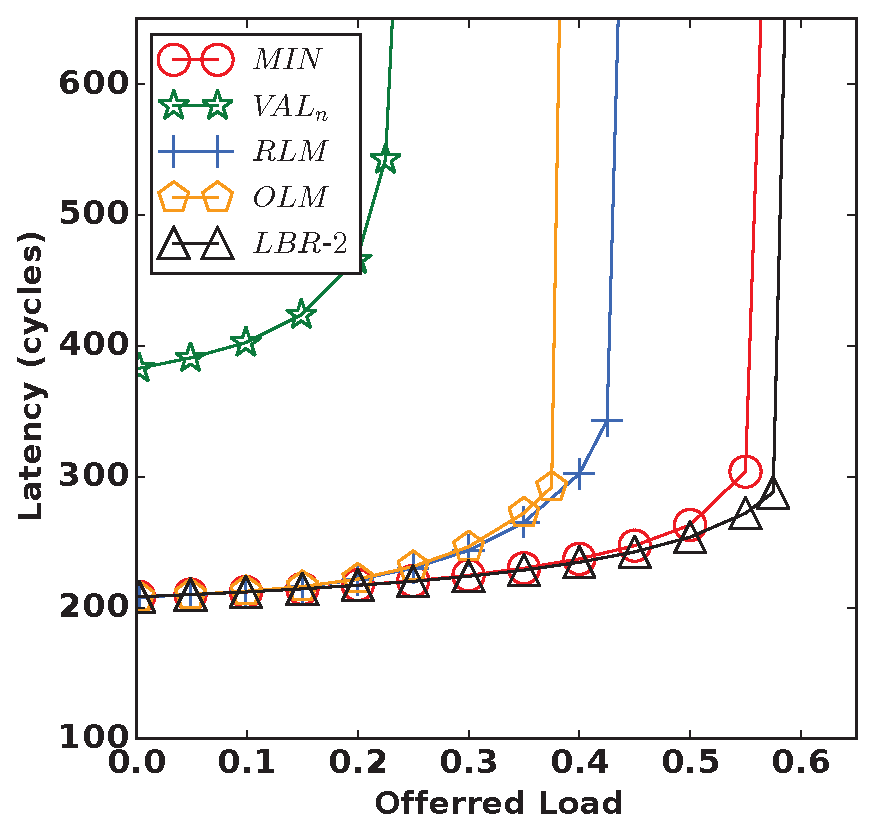
\includegraphics[width=.40\textwidth,height=.42\textwidth]{latency16flit2pattern0.eps}
    \label{latency16flit2pattern0}
  }
  \subfloat[Adversarial]{
    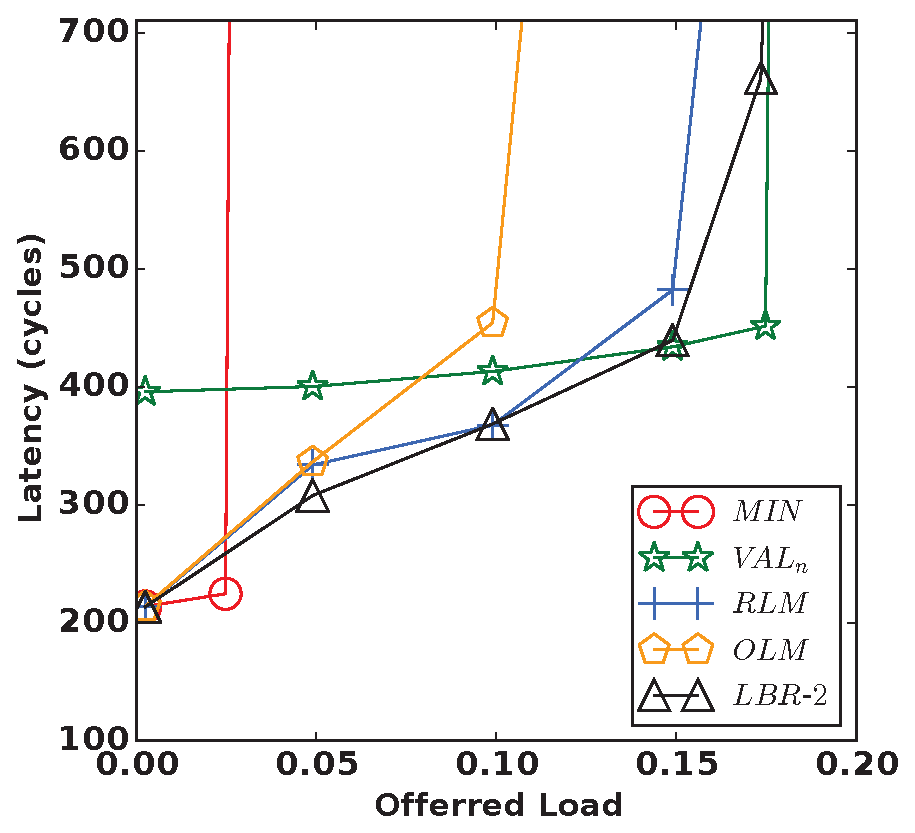
\includegraphics[width=.40\textwidth,height=.42\textwidth]{latency16flit2pattern1.eps}
    \label{latency16flit2pattern1}
  }
  \caption{报文长度为16个切片的延迟}
  \label{fig:latency16flits}
  \end{minipage}
  \end{figure*}

  \subsection{VC分配策略}

  在有多条VC的条件下,LBR算法中允许绿色报文没有限制的选择不同的VC。
  我们提出三种选择VC的策略,分别是Random、Mod-Minimal以及Minimal。
  Mod-Minimal是默认的VC分配策略,如算法\ref{algo:va}所示。在混合通信
  模式下,分别在LBR-2和LBR-3两种路由算法上模拟了这三种分配策略,如图\ref{fig:vcstrategies}
  所示。Random策略的延迟最低,是因为每次都选最短的VC队列,可以减少排队时间。
  但是,Mod-Minimal策略的饱和吞吐率最高则是因为这是一个均衡的缓冲区使用机制,
  根据报文的状态并结合VC队列长度来选择合适VC队列,一定程度上对报文做了划分
  降低了头阻塞的概率。


    \begin{figure*}[t]
     \centering
    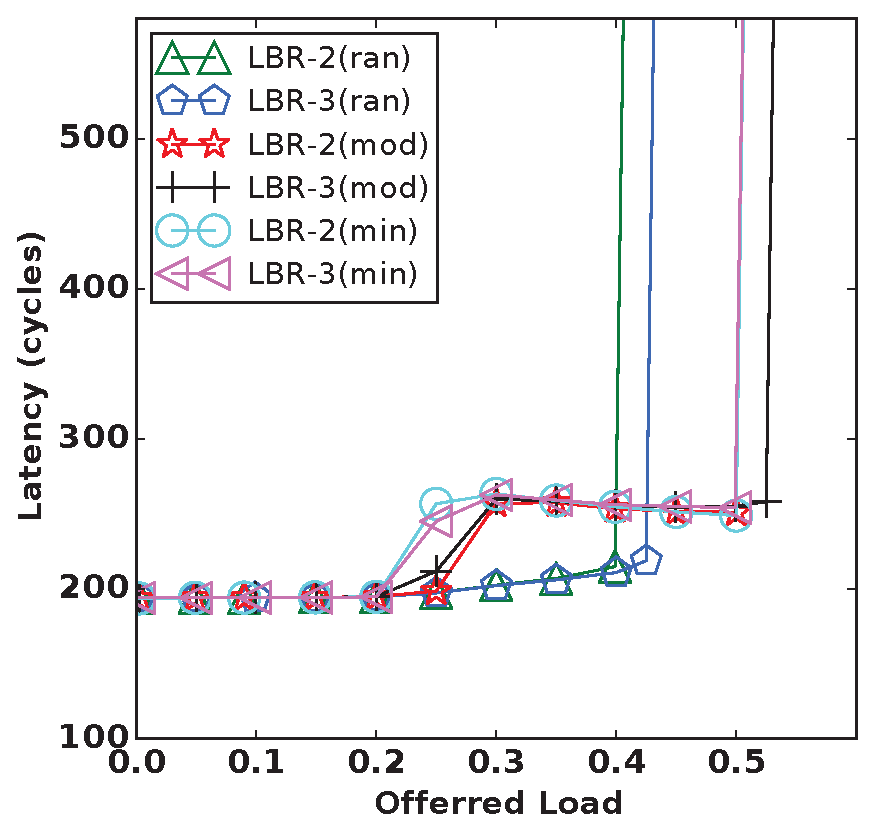
\includegraphics[width=.5\textwidth]{latencyGRR2vc3vcblend.eps}
  \caption{混合通信模式下VC分配策略性能比较}
  \label{fig:vcstrategies}

\end{figure*}


  \subsection{本章小结}

  在本章工作中,我们提出了一个新的基于标签的大规模低直径高性能互连网络路由算法,LBR。
  LBR采用一种新的、有效的缓冲区组织方式LBBO来解决死锁避免开销和路由自适应性的
  权衡问题。LBR降低了自适应路由对VC数量的要求,并有效降低死锁避免的开销,只需要一个报文
  大小的缓冲区。LBR是一个不同于传统使用多条VC的路由算法,但是,在端口有多条VC的条件下,
  LBR也能充分利用VC资源来提升网络性能。LBR均衡使用缓存资源的利用率并支持完全自适应路由
  算法。详细的实验结果展示了LBR在大多数通信模式下都优于别的路由算法。


  \begin{comment}
  \subsection{缓冲区划分}

  在这一节中,我们比较了两种缓冲区划分策略:(1)Single策略:$VC_0$中存放
  红色报文的队列大小为1个报文大小。(2)Half策略:$VC_0$中存放红色报文的队列
  大小为$VC_0$缓冲区大小的一半。我们设置了两种全局端口缓冲区配置,一种是256个
  切片大小,一种是128切片大小。因此,我们有四种情况进行分析比较:

  \begin{figure*}
 \centering
  \begin{minipage}[t]{\textwidth}
  \subfloat[Latency]{
    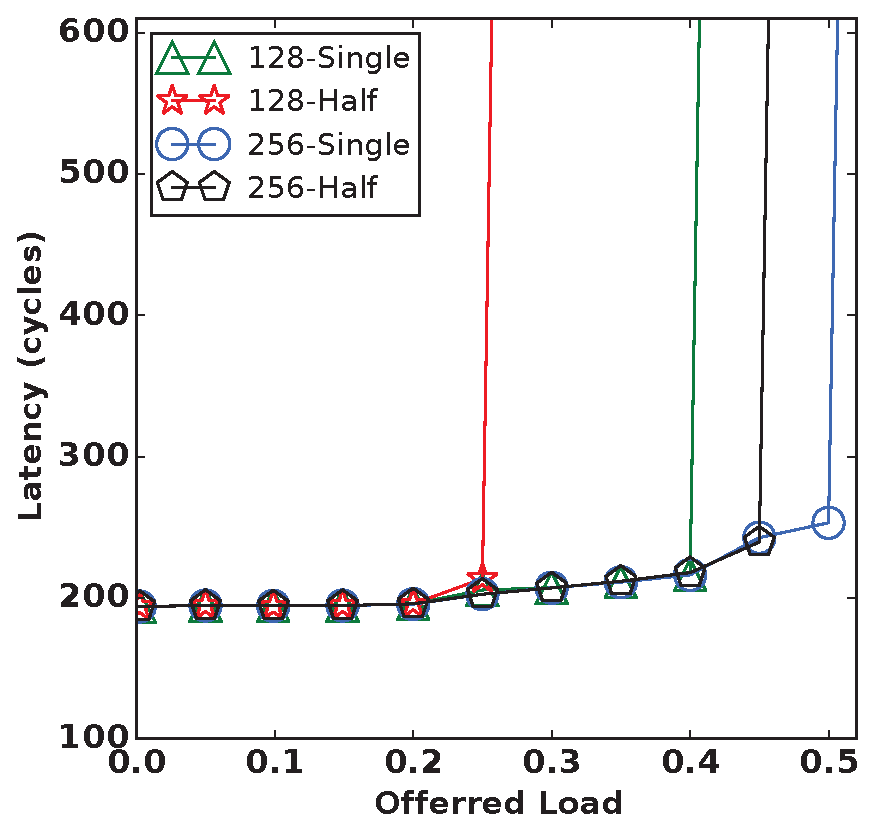
\includegraphics[width=.28\textwidth,height=.3\textwidth]{latencygrr1vcescape2vcblend.eps}
    \label{latencygrr1vcescape2vcblend}
  }
  \subfloat[Routing Computation]{
    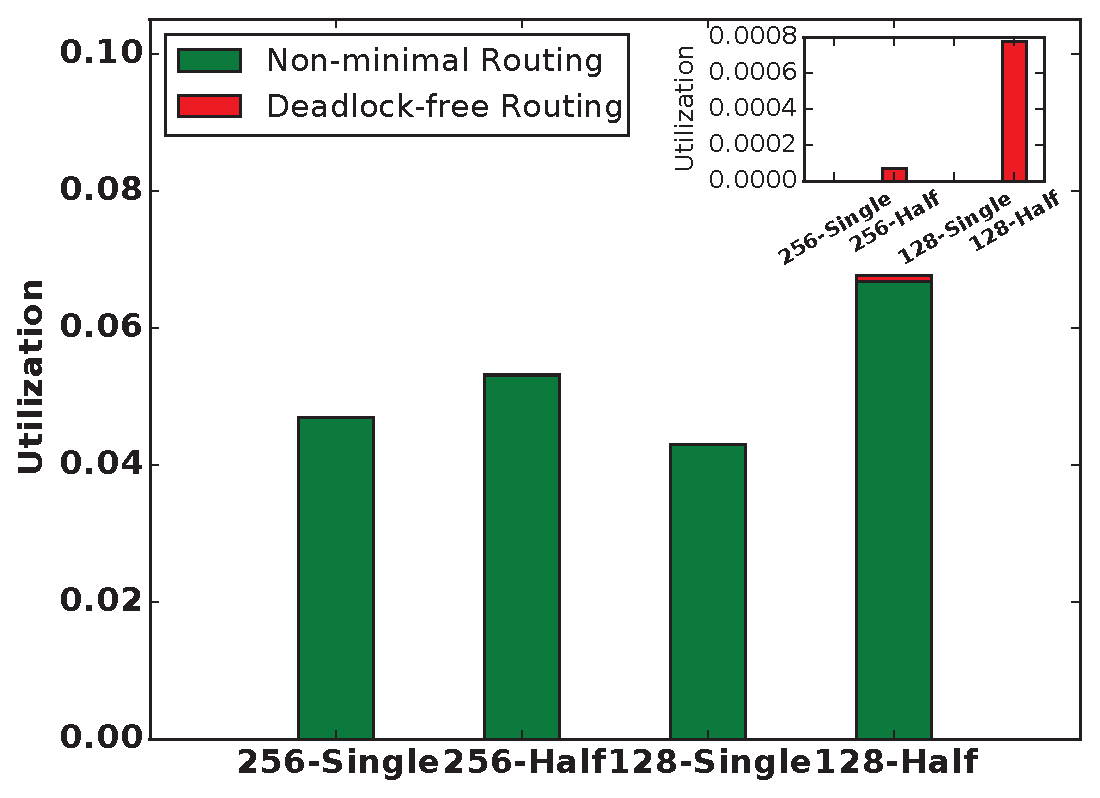
\includegraphics[width=.28\textwidth,height=.3\textwidth]{rcgrr1vcescape2vcblenddlf.eps}
    \label{rcgrr1vcescape2vcblenddlf}
  }
  \subfloat[VC Utilization]{
    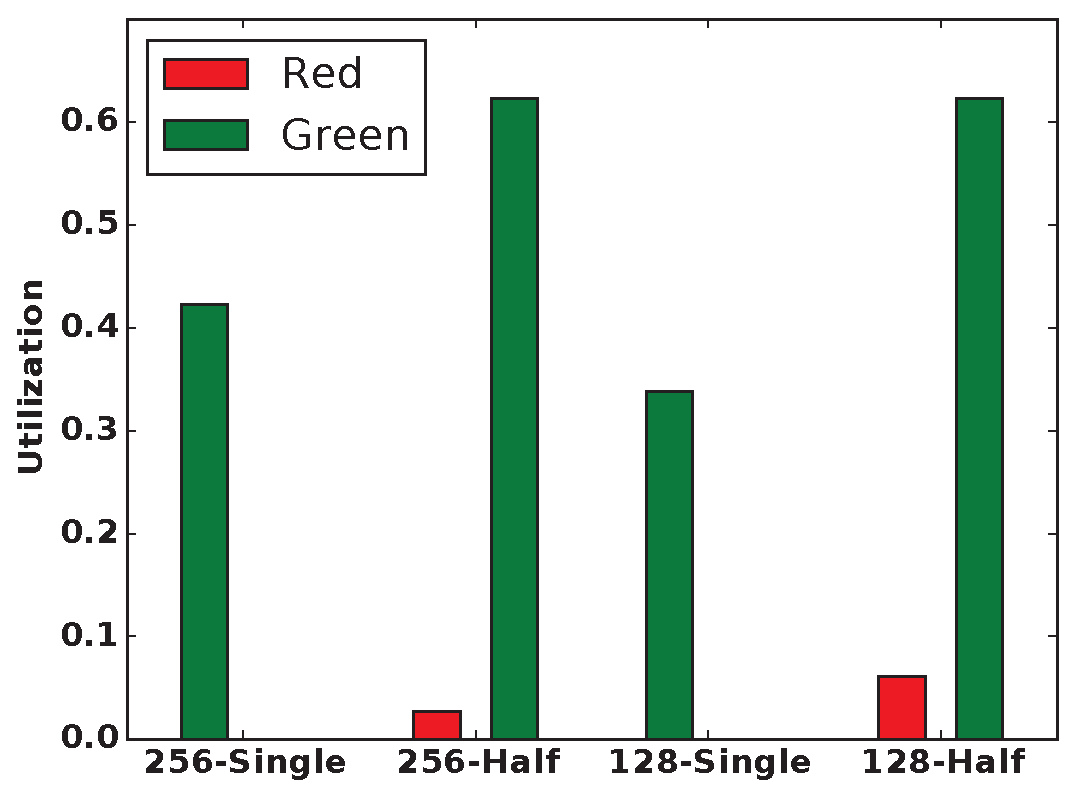
\includegraphics[width=.28\textwidth,height=.3\textwidth]{vcgrr1vcescape2vcblenddlf.eps}
    \label{vcgrr1vcescape2vcblenddlf}
  }
  \caption{Buffer Partitioning under Blended Traffic Pattern}
  \label{fig:grr1escape2blend}
  \end{minipage}
\end{figure*}

  \begin{figure*}
 \centering
  \begin{minipage}[t]{\textwidth}
  \subfloat[Latency]{
    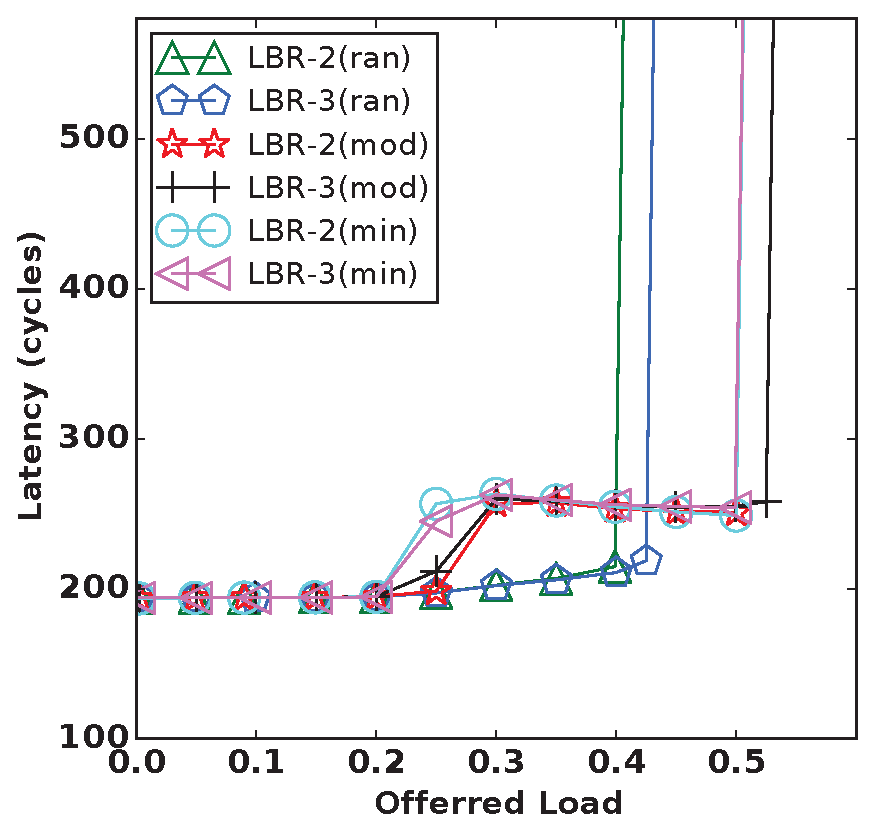
\includegraphics[width=.28\textwidth,height=.3\textwidth]{latencyGRR2vc3vcblend.eps}
    \label{latencyGRR2vc3vcblend}
  }
  \subfloat[GRR-2]{
    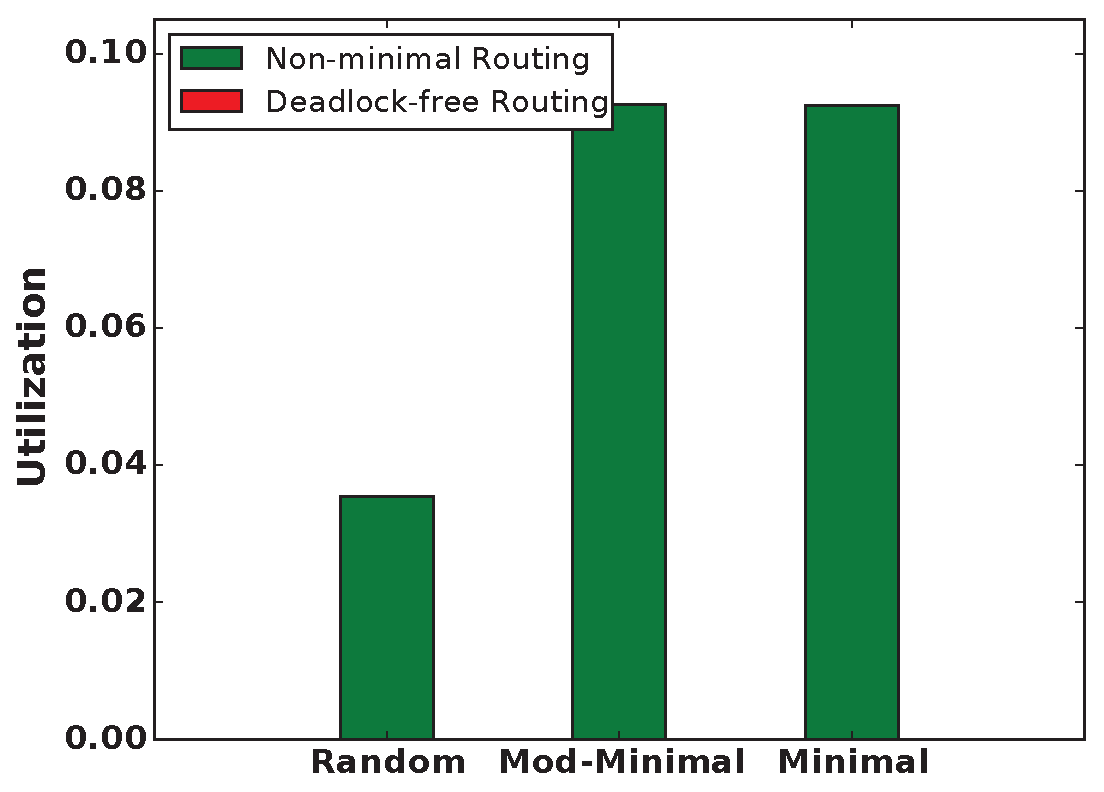
\includegraphics[width=.28\textwidth,height=.3\textwidth]{latencyGRRunad2vcrcblend.eps}
    \label{latencyGRRunad2vcrcblend}
  }
  \subfloat[GRR-3]{
    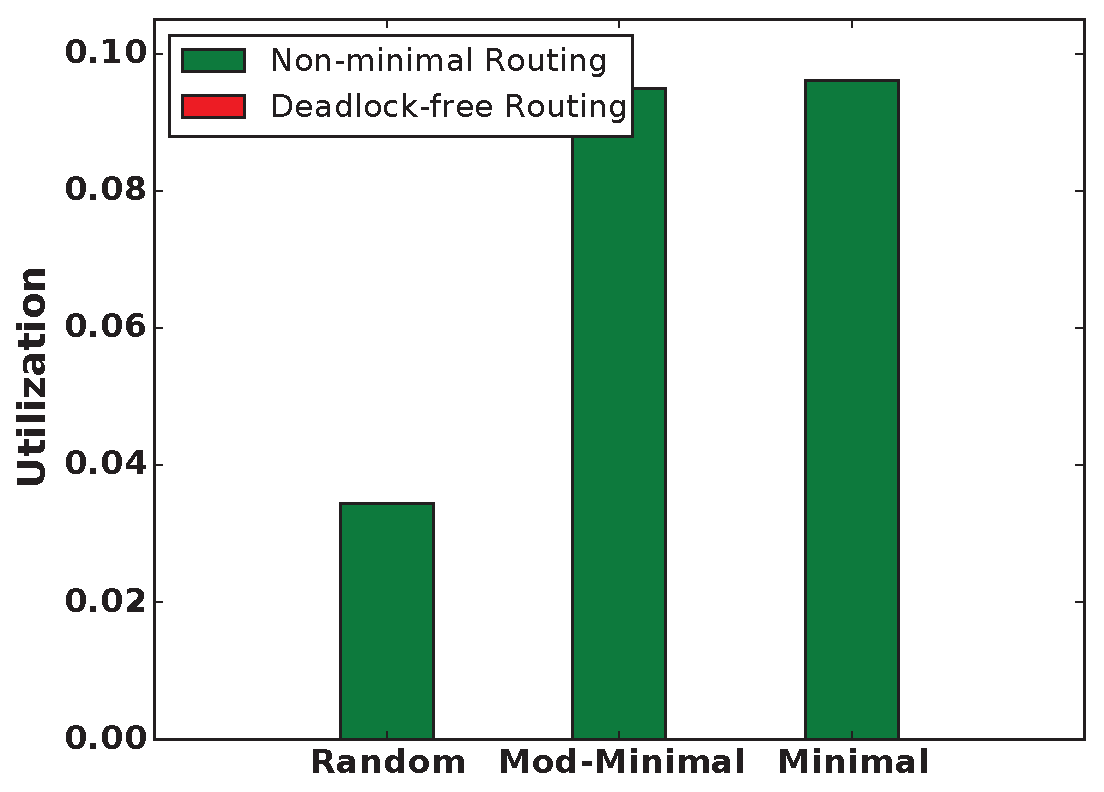
\includegraphics[width=.28\textwidth,height=.3\textwidth]{latencyGRRunad3vcrc.eps}
    \label{latencyGRRunad3vcrc}
  }
  \caption{VC Allocation Strategies under Blended Traffic Pattern}
  \label{fig:vcstrategies}
  \end{minipage}
\end{figure*}

\end{comment}
